\documentclass[40pt,letterpaper,physrev]{article}
\usepackage[utf8]{inputenc}
\usepackage{float}
\usepackage{graphicx}
\usepackage{graphics}
\usepackage{amsmath}
\usepackage{amsfonts}
\usepackage{amssymb}
\usepackage{cancel}
\usepackage{times} % set times font
\usepackage{color}
\usepackage{datetime}
\usepackage{fullpage}
\usepackage{tikz}
\usepackage{caption}
\DeclareGraphicsExtensions{.pdf,.png,.jpg,.eps} 
\author{Dmitri Priimak}
\title{High-frequency signal amplification in semiconductor super-lattice in cross electric and magnetic fields}
\begin{document}
\bibliographystyle{plain}
\newcommand{\ddx}[2] {
	\frac{\text{d}#1}{\text{d}#2}
}
\newcommand{\ddt}[1] {
	\frac{\text{d}#1}{\text{d}t}
}
\newcommand{\dtwodt}[1] {
	\frac{\text{d}^{2}#1}{\text{d}t^{2}}
}
 \begin{center}
  \underline{High-frequency signal amplification in semiconductor super-lattice in cross electric and magnetic fields}
 \end{center}
  \begin{center}
    \underline{Rev. 17}
  \end{center}
  \section{Introduction}  
  A semiconductor superlattice (SL), first studied by Esaki and Tsu \cite{Esaki:70}, offers may opportunities for
  industrial 
  applications, some of which has been realized [*] and some are still waiting to be discovered. One of the
  earliest studied properties of SL were Bloch oscillations \cite{BLOCH}, which would allow amplification of 
  THz emf fields. This however did not come to fruition as there are mechanisms that destroy these 
  oscillations, one of
  which is formation of electron domains [*]. However 
  tell-tale signs of Bloch oscillations were detected in experiments where transient processes of electron 
  relaxation were studied in SL \cite{PhysRevB.56.10303}. Several different methods to stabilise Bloch oscillations were proposed [*], 
  but experimental verification proves elusive [*]. Detailed review of SL theory and known analytical solutions 
  can be found in work by A. Wacker \cite{WAC01}.
  
  In out work we look at SL, using semi-classical theory, under action of electric field $E(t)=E_{dc}+E_\omega\cos(\omega t)$ along the 
  superlattice axis and constant perpendicular magnetic field.
  	\begin{figure}[H]
	  \centering
	  \normalsize % use normal font size in the figure
	  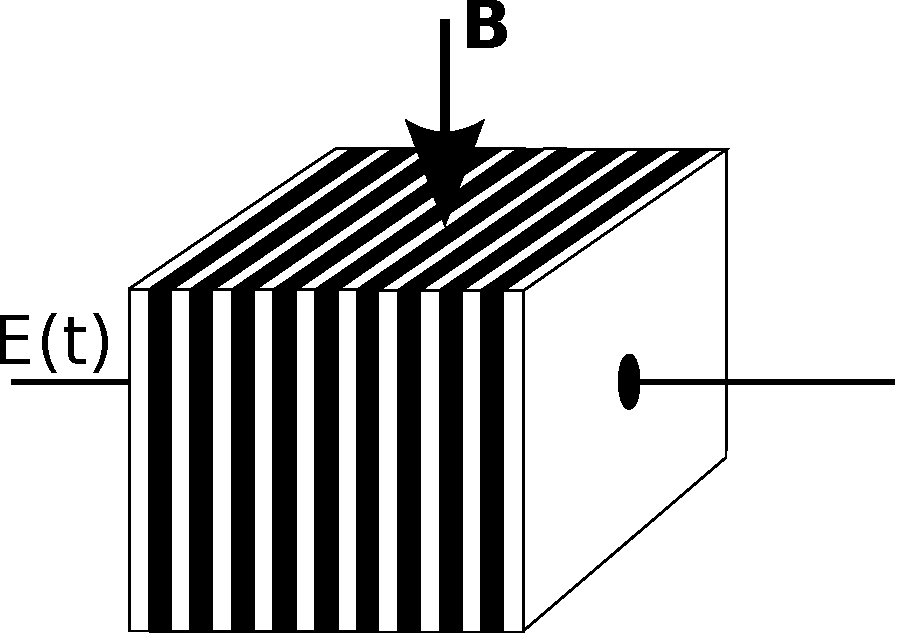
\includegraphics[scale=0.7]{illustrations/SL_CROSS_E_AND_B.pdf}
	  \caption{}
	\end{figure}
  This configuration has already been studied in the limiting case of zero temperature \cite{PhysRevLett.103.117401}. We, however, will be 
  looking at non-zero temperature, all the way up to the room temperature. The gist of our approach is that we 
  will be looking at such values of $B$ and $E_{dc}$ so that SL does not operate in Bloch oscillation regime, but
  instead is in cyclotron like mode. This way we can avoid stability problems inherent in Bloch oscillations and 
  non-linearity of dispersion relation provides possibility of small, high frequency signal amplification, 
  ultimately paving the way to the lasing medium.
  
  \section{Analytical treatment}
    We take approach of semi-classical theory based on Boltzmann equation, where, the entirety of quantum 
    mechanical nature of the SL is hidden in electron velocity $\mathbf{v}(\mathbf{k})$, which is a function of $
    \mathbf{k}$, crystal momentum. 
    \begin{equation}\label{eq:boltzmann}
     \frac{\partial f}{\partial t}+
     \frac{e}{\hbar}\left ( \mathbf{E} + \mathbf{v}\times\mathbf{B} \right ) \frac{\partial f}{\partial\mathbf{k}}+
     \mathbf{v}(\mathbf{k})\frac{\partial f}{\partial r} = \left ( \frac{\partial f}{\partial t} \right )_{st}
    \end{equation}
    Where $\left ( \partial f/\partial t \right )_{st}$ is a collision term responsible for relaxation to the
    normal electron density distribution function in the absence of external fields. Here we consider the simplest
    form of this term $(f_0-f)/\tau$. Where $f_0$ is, in general, Fermi distribution, but at finite temperatures
    can be approximated by Boltzmann distribution.
    Since we consider electron density $f$ to be spatially homogeneous, $f$ depends only on $\mathbf{k}$ and 
    Boltzmann equation takes form
    \begin{equation}\label{eq:boltzmann_homo}
     \frac{\partial f}{\partial t}+
     \frac{e}{\hbar}\left ( \mathbf{E} + \mathbf{v}\times\mathbf{B} \right ) \frac{\partial f}{\partial\mathbf{k}}
     = \frac{f_0 - f}{\tau}
    \end{equation}
    Electric field is along x-axis and magnetic field is along z-axis.
    \begin{align}
     \mathbf{E}=&(E,0,0) \\
     \mathbf{B}=&(0,0,B) \\
     \mathbf{v}\times\mathbf{B}=&(v_y B, -v_x B, 0))
    \end{align}
    We now proceed with making variety of substitutions to turn this equation into dimensionless form. First we
    will make following substitution
    \begin{equation}
     t \to \tau t
    \end{equation}
    which gives following form to the Boltzmann equation
    \begin{equation}
     \frac{\partial f}{\partial t}+
     \frac{ed\tau}{\hbar}(E+v_{y}B)\frac{\partial f}{\partial(k_x d)}-
     \frac{ed\tau}{\hbar}v_{x}B\frac{\partial f}{\partial(k_y d)}
     = f_0 - f
    \end{equation}
    where 
    \begin{equation}
     \mathbf{v}=\frac{1}{\hbar}\frac{\partial\varepsilon}{\partial\mathbf{k}}
    \end{equation}
    and $\varepsilon$ is an energy of an electron in the zone, which in tight-binding apporiximation takes form in the first zone
    \begin{equation}
     \varepsilon=\frac{\hbar^2k^2_y}{2m}-\frac{\Delta_{1}}{2}\cos(k_{x}d)\label{eq:energy_unscaled}
    \end{equation}
    therefore
    \begin{align}
     v_x=&\frac{\Delta_{1}d}{2\hbar}\sin(dp_x/h) \\
     v_y=&\frac{\hbar k_y}{m}
    \end{align}
    And Boltzmann equations now takes following form
   \begin{equation}
     \frac{\partial f}{\partial t}+
     \left ( \frac{ed\tau}{\hbar}E+\frac{ed\tau}{m}k_yB \right ) \frac{\partial f}{\partial(k_x d)}-
     \frac{\Delta_{1}ed^2\tau}{2\hbar^2}B\sin(k_{x}d)\frac{\partial f}{\partial(k_y d)}
     = f_0 - f
   \end{equation}
   Now we can define
   \begin{align}
	E_*=&\frac{\hbar}{ed\tau} \\	
	m_x=&\frac{2\hbar^2}{\Delta_1 d^2} \\
   \end{align}
   \begin{equation}
	\boxed{\alpha=m/m_x}
   \end{equation}
   Then, with cyclotron frequency defined as 
   \begin{equation}
	\omega_c=\frac{eB}{\sqrt{mm_x}}
   \end{equation}
   we get following
   \begin{equation}
     \frac{\partial f}{\partial t}+
     \left ( \frac{E}{E_*}+\frac{\omega_{c}\tau}{\sqrt{\alpha}}k_yd \right ) \frac{\partial f}{\partial(k_x d)}-
     \sqrt{\alpha}\omega_c\tau\sin(k_x d)\frac{\partial f}{\partial(k_y d)}
     = f_0 - f
   \end{equation}
   And if we now define
   \begin{align}
       \phi_x=&k_{x}d \\
       \phi_y=&\frac{k_{y}d}{\sqrt{\alpha}} \\
       \tilde{E}=&E/E_*\\
       \tilde{B}=&\omega_{c}\tau
   \end{align}
   Boltzmann equations takes form
   \begin{equation}
   	\boxed{
   	\label{eq:boltzmann_final}
     \frac{\partial f}{\partial t}+
     \left ( \tilde{E}+\tilde{B}\phi_y\right ) \frac{\partial f}{\partial\phi_x}-
     \tilde{B}\sin(\phi_x)\frac{\partial f}{\partial\phi_y}
     = f_0 - f}
   \end{equation}
   Alternatively, if we define Bloch frequency as
   \begin{equation}
	\omega_B=\frac{edE}{\hbar}
   \end{equation}
   it can be written as 
   \begin{equation}
     \frac{\partial f}{\partial t}+
     \left ( \omega_B\tau+\omega_c\tau\phi_y\right ) \frac{\partial f}{\partial\phi_x}-
     \omega_c\tau\sin(\phi_x)\frac{\partial f}{\partial\phi_y}
     = f_0 - f
   \end{equation} 
    Ratio of Bloch and cyclotron oscillation frequencies will be important to us down the road.
    For $f_0$ we use Boltzmann distribution 
    \begin{equation}
        f_0\propto e^{\displaystyle -\frac{\varepsilon}{k_bT}}
    \end{equation}
    which in our variables $\phi_x$ and $\phi_y$ takes form
    \begin{equation}
	f_0=C\exp{\left \{ \mu\cos(\phi_x)-\frac{\mu}{2}\phi^2_y\right \} }
	\end{equation}
	\begin{equation}
	\boxed{\mu=\frac{\Delta_1}{2k_{b}T}}
    \end{equation} 
    Now, constant $C$ must be such that dimensionless norm of $f_0$ is 1. Therefore
    \begin{align}
       \frac{1}{C}=&\frac{d^2}
	{\hbar^2}\int^{+\infty}_{-\infty}\text{d}p_y\int_{p_x\in\text{BZ}}\text{d}p_x
	\exp{\left \{ \mu\cos(\phi_x)-\frac{\mu}{2}\phi^2_y\right \} } \\
	   =&\sqrt{\alpha}\int^{+\infty}_{-\infty}e^{-\mu\phi^2_y/2}\text{d}\phi_y
	   \int^{\pi}_{-\pi}e^{\mu\cos(\phi_x)}\text{d}\phi_x \\
	   =&2\pi I_0(\mu)\sqrt{\frac{2\pi\alpha}{\mu}}
    \end{align}
    Thus, full form of equilibrium distribution is
    \begin{equation}
    \boxed{
	f_0=\frac{1}{2\pi I_0(\mu)}\sqrt{\frac{\mu}{2\pi\alpha}}\exp{\left \{ \mu\cos(\phi_x)-\frac{\mu}{2}\phi^2_y\right \} } }
	\end{equation}
	This way, in total, we have four free parameters defining our system, $\mu$ and $\alpha$ that characterize lattice parameters such as lattice period and band width and temperature, and $\tilde{E}$, $\tilde{B}$ that specify external fields.
	One of the parameters that we will be calculating is drift 
	velocity $v_{dr}$, which we will define like this
	\begin{align}
		v_{dr}=&\frac{2d}{\Delta_1\hbar}\iint
			\frac{\partial\varepsilon}{\partial p_x}f(p_x,p_y)\text{d}p_x\text{d}p_y \\
			=&\sqrt{\alpha}\int^{\pi}_{-\pi}\text{d}\phi_x\int^{+\infty}_{-\infty}\text{d}\phi_y\sin(\phi_x)f(\phi_x,\phi_y)\label{eq:v_dr_generic}
	\end{align}
    When magnetic field is $0$ and $E$ is constant, i.e. $E_{dc}$, analytic 
    solution Boltzmann equation is well known and as well as expression for 
    drift velocity and absorption (see below) \cite{WAC01}
    \begin{align}
	v_{dr}=&\left \{ \sqrt{\alpha}\int^{\pi}_{-\pi}\text{d}\phi_x\int^{+\infty}_{-\infty}\text{d}\phi_y\sin(\phi_x)f_0(\phi_x,\phi_y)\right \}
	\frac{E_{dc}/E_*}{1+(E_{dc}/E_*)^2} \\
	=&\frac{I_1(\mu)}{I_0(\mu)}\frac{E_{dc}/E_*}{1+(E_{dc}/E_*)^2}
    \end{align}
	From which follows that peak value of $v_{dr}$ is at $E_{dc}/E_*=1$ and is 
	\begin{equation}
		v_p=\frac{I_1(\mu)}{2I_0(\mu)}\label{eq:v_peak}
	\end{equation}
	Later, down the road, we will be plotting not $v_{dr}$, but $v_{dr}/v_p$,
	which for dc electric field only take very simple form, known as "Esaki-Tsu" equation
	\begin{equation}
		\frac{v_{dr}}{v_p}=2\frac{E_{dc}/E_*}{1+(E_{dc}/E_*)^2}
	\end{equation}
	In general we will be applying a/c emf in the form 
	\begin{equation}
	\tilde{E}=\tilde{E}_{dc}+\tilde{E}_{\omega}\cos(\omega t)\label{eq:tilde_E_as_a_function_of_time}
	\end{equation}
	and in case when magnetic field is not applied we also have analitic expression for $v_{dr}$, which is known as "Tien-Gordon" equation. Analytic expression, "Taker formulae", is also known for absorption, which we will define like this
	\begin{equation}
	A=\left <\frac{v_{dr}}{v_p}\cos(\omega t) \right >_{t}
	\end{equation}
	In case when magnetic field is appied, however, analytic expression for absorption is not known. And that is the quantity we are most interested in.
	
	Now due to periodicty of $f(\phi_x,\phi_y)$ along $\phi_x$ with 
	period $2\pi$ and additionally 
	$f_0(-\phi_x, \phi_y)=f_0(\phi_x, \phi_y)$, it makes sense 
	for us to expand $f$ and $f_0$ into Fourier series.
	\begin{align}
		f_0=&\sum^\infty_{n=0}a^{(0)}_{n}\text{cos}(n\phi_x)\label{eq:f0_fourier_representation} \\
		f=&\sum^\infty_{n=0}a_{n}\text{cos}(n\phi_x)+
		b_{n}\text{sin}(n\phi_x)\label{eq:f_fourier_representation}
	\end{align}
	where coeffients $a^{(0)}_n$, $a_n$ and $b_n$ in general will depend on $\phi_y$ and last two also on time $t$. Note, that $a_{n<0}\equiv 0$ and $b_{n<1}\equiv 0$. And with the from of $f_0$, as selected above, $a^{(0)}_n$ becomes
	\begin{align}
		a^{(0)}_n=&\frac{\sigma(n)}{\pi}\int^{\pi}_{-\pi}f_0(\phi_x,\phi_y)\cos(n\phi_x)\text{d}\phi_x \\
		=&\frac{\sigma(n)I_n(\mu)}{\pi I_0(\mu)}\sqrt{\frac{\mu}{2\pi\alpha}}\exp{\left \{ -\frac{\mu}{2}\phi^2_y\right \} }
	\end{align}
	where 
	\begin{equation}
		\sigma(n)=
		\begin{cases}
   		1/2 & : n=0 \\
   		1 & : n\ne 1
  		\end{cases}
	\end{equation}
	Norm of $f(\phi_x,\phi_y)$ must always be one, i.e.
	\begin{equation}
		\sqrt{\alpha}\int^{\pi}_{-\pi}\text{d}\phi_x
			\int^{+\infty}_{-\infty}\text{d}\phi_y f(\phi_x,\phi_y)=1
	\end{equation}
	which in fourier representation takes form
	\begin{equation}
	\boxed{
		2\pi\sqrt{\alpha}\int^{+\infty}_{-\infty}a_0(\phi_y)\text{d}
		\phi_y=1}
	\end{equation}
	Once we move on to the numerical calculations this equation can be used to check correctness. And from equation (\ref{eq:v_dr_generic}) it is clear that only $b_1$ will survice. And calculation of $v_{dr}$ is done through following 
	equation
	\begin{align}
		v_{dr}=&\sqrt{\alpha}\int^{+\infty}_{-\infty}\text{d}\phi_{y}\int^{+\pi}_{-\pi}\text{d}\phi_x\sin(\phi_x)b_1(\phi_y)\sin(\phi_y)\\
		=&\pi\sqrt{\alpha}\int^{+\infty}_{-\infty}b_1(\phi_y)\text{d}\phi_y
	\end{align}
	and in view of definition of peak value of $v_{dr}$ in eq. (\ref{eq:v_peak})
	\begin{equation}
	\boxed{
		\frac{v_{dr}}{v_p}=\frac{2I_0(\mu)\pi\sqrt{\alpha}}{I_1(\mu)}
			\int^{+\infty}_{-\infty}b_1(\phi_y)\text{d}\phi_y
			}
	\end{equation}
	In addition to drift velocity along $x$-axis we can look at drift velocity alogn $y$-axis, which we will define like this
	\begin{align}
	v_y=&\frac{2}{\Delta_1}\iint\frac{\partial\varepsilon}{\partial p_y}f(\phi_x,\phi_y)\text{d}p_x\text{d}p_y \\
	=&\int^{\pi}_{-\pi}\text{d}\phi_x\int^{+\infty}_{-\infty} \phi_y f(\phi_x,\phi_y) \text{d}\phi_y \\
	=&2\pi\int^{+\infty}_{-\infty}a_0(\phi_y)\phi_y\text{d}\phi_y
	\end{align}
	However just as with drift velocity along $x$-axis we will be working with ratio of $v_y$ and peak velocity $v_p$.
	\begin{equation}
	\boxed{
	\frac{v_y}{v_p}=\frac{4\pi I_0(\mu)}{I_1(\mu)}\int^{+\infty}_{-\infty}a_0(\phi_y)\phi_y\text{d}\phi_y
	}
	\end{equation}
	This way we accounted for meaning of $a_0$ and $b_1$. Let us now take a look at $a_1$. Effective mass of an electron in the $x$ direction is given by 
	\begin{equation}
		m^{-1}_{x,\mathbf{k}}=\frac{1}{\hbar^2}\frac{\partial^2\varepsilon}{\partial k^2_x}
	\end{equation}
	Negative sign of electron effective mass can serve as an intuitive indicator of such state of the system,
	where a/c signal amplification is possible. Although in more exotic situations amplification may take place
	even with positive sign of electron effective mass. In out calculations, however, we will be working with
	ratio of electron mass to $m_{x,\mathbf{k}}$. And in tight-binding approximation, when 
	energy is defined as (\ref{eq:energy_unscaled}), that takes form
	\begin{align}
	\frac{m}{m_{x,\mathbf{k}}}=&\frac{\Delta_1 d^2m}{2\hbar^2}\cos(k_xd) \\
	=&\alpha\cos(\phi_x)
	\end{align}
	To gather back this value from $f(\phi_x,\phi_y)$ we have to integrate over $\{p_x,p_y\}$ and to maintain dimensionlessness of ratio of these masses, this integration will take form
	\begin{align}
	\frac{m}{m_{x,\mathbf{k}}}=&\alpha^{3/2}\frac{d^2}{\hbar^2}\iint f(\phi_x, \phi_y)\cos(k_{x}d)\text{d}p_x\text{d}p_y \\
	=&\alpha^{3/2}\int^{\pi}_{-\pi}\text{d}\phi_x\int^{+\infty}_{-\infty}\text{d}\phi_y f(\phi_x, \phi_y)\cos(\phi_x) \\
	=&\alpha^{3/2}\int^{\pi}_{-\pi}\text{d}\phi_x\int^{+\infty}_{-\infty}\text{d}\phi_y a_1(\phi_y)\cos(\phi_x)\cos(\phi_x)
	\end{align}
	Finally giving us following
	\begin{equation}
	\boxed{
		\frac{m}{m_{x,\mathbf{k}}}=\pi\alpha^{3/2}\int^{+\infty}_{-\infty} a_1(\phi_y)\text{d}\phi_y
		}
	\end{equation}
	Now using fourier representation of $f(\phi_x,\phi_y)$ and $f_0(\phi_y)$ (equations \ref{eq:f0_fourier_representation}, \ref{eq:f_fourier_representation}) we can rewrite Boltzmann equation (\ref{eq:boltzmann_final}) like this
	\begin{align}
	&\sum_{(n)}\bigg \{ \frac{\partial a_n}{\partial t}\cos(n\phi_x) + \frac{\partial b_n}{\partial t}\sin(n\phi_x) = a^{(0)}_{n}\cos(n\phi_x)-a_n\cos(n\phi_x)-b_n\sin(n\phi_x)+\nonumber \\
	&n(\tilde{E}+\tilde{B}\phi_y)(a_n\sin(n\phi_x)-b_n\cos(n\phi_x))+ \tilde{B}\frac{\partial a_n}{\partial\phi_y}\sin(\phi_x)\cos(n\phi_x) + \tilde{B}\frac{\partial b_n}{\partial\phi_y}\sin(\phi_x)\sin(n\phi_x)\bigg \}
	\end{align}
	In absence of magnetic field there is no mixing of different harmonic, however when $\tilde{B}$ is not $0$ then harmonics will be come mixed due to presence of $\sin(\phi_x)\cos(n\phi_x)$ and $\sin(\phi_x)\sin(n\phi_x)$, since
	\begin{align}
	\sin(\phi_x)\cos(n\phi_x)=&\left \{ \sin((n+1)\phi_x) -\sin((n-1)\phi_x) \right \}/2 \\
	\sin(\phi_x)\sin(n\phi_x)=&\left \{ \cos((n-1)\phi_x) -\cos((n+1)\phi_x) \right \}/2
	\end{align}
	And using this equations, after some manipultion of symbols,
	combining elements with the same harmonics, and noting special treatment of $b_1$ we get
	\begin{align}
		\frac{\partial a_n}{\partial t}=&a^{(0)}_n-a_n-n(\tilde{E}+\tilde{B}\phi_y)b_n+\tilde{B}\left ( \frac{\partial b_{n+1}}{\partial\phi_y}-\frac{\partial b_{n-1}}{\partial\phi_y} \right )\label{eq:a_n_dot} \\
		\frac{\partial b_n}{\partial t}=&-b_n-n(\tilde{E}+\tilde{B}\phi_y)a_n+\tilde{B}\left ( \chi(n)\frac{\partial a_{n-1}}{\partial\phi_y}-\frac{\partial a_{n+1}}{\partial\phi_y} \right ) \label{eq:b_n_dot}
	\end{align}
	where
	\begin{equation}
		\chi(n)=
		\begin{cases}
	   2 & : n= 1 \\
	   1 & : n\ne 1
	  \end{cases}
	\end{equation}
    \section{Correspondence with classical pendilum}
    In the limit where dissipation is absent instead of Boltzmann
    equation we can use semiclassical equations of motion working 
    individual electrons. Such situation corresponds to $\tau=\infty$ and initial shape of $f(\phi_x,\phi_x)$ being delta function. 
    \begin{align}
    	\hbar\frac{\text{d}\mathbf{k}}{\text{d}t}=&e\mathbf{E}+e\mathbf{v}\times\mathbf{B} \\
    	\mathbf{v}(\mathbf{k})=&\frac{1}{\hbar}\frac{\partial\varepsilon}{\partial\mathbf{k}}
    \end{align}
    And in view of specific values of $\mathbf{E}$, $\mathbf{B}$ and $\varepsilon$ that we are using in our problem, these equations transform into following
    \begin{align}
	    \ddt{\phi_x}=&\tilde{E}+\tilde{B}\phi_y \label{eq:semi_classical_phi_x_dot} \\
	    \ddt{\phi_y}=&-\tilde{B}\sin(\phi_x) \label{eq:semi_classical_phi_y_dot}
    \end{align}
    And taking second derivative of (\ref{eq:semi_classical_phi_x_dot}), assuming that $\tilde{E}$ is defined by (\ref{eq:tilde_E_as_a_function_of_time}) we arrive to second order ODE, which correspond to classical externally driven pendilum.
    \begin{equation}
    	\dtwodt{\phi_x}+\tilde{B}^2\sin(\phi_x)=-\omega\tilde{E}_\omega\sin(\omega t)
    \end{equation}
    In general this equation can exibit very complicated behaviour and even chaos, but can be solved in the simplest case when $\tilde{E}_\omega=0$, in which case peroid of oscillation is defined by magnetic field $\tilde{B}$ and electric field $\tilde{E}$, which sets initial velocity of $\phi_x$, i.e. $\ddt{\phi_x}$ at $t=0$, assuming that $\phi_x$ and $\phi_y$ at $t=0$ are also $0$. In case of $E_\omega=0$ we exact correspondence of our system to a classical pendilum, for which 
    we do have conservation of energy.
    \begin{equation}
    \frac{1}{2}\left ( \ddt{\phi_x} \right  )^2+2\tilde{B}^2\sin^2(\phi_x/2)=E_{total}
    \end{equation}
    If we define $E_p=2\tilde{B}^2$, which corresponds to 
    "peak" then when $E_{total}=E_p$ then such pendilum can reach 
    inverted position. When $\phi_x$ and $\phi_y$ are equal zero 
    $E_{total}=\tilde{E}_{dc}^2/2$ and thus for $E_p$ there is 
    corresponding $E_{sx}=2\tilde{B}$, which defines separatrix dividing
    motion of the pendilum between vibrational 
    ( $\tilde{E}_{dc}<E_{sx}$ ) and 
    rotational ( $\tilde{E}_{dc}>E_{sx}$ ).
    When our system gives peak of negative absorption corresponding 
    to the first and second cases we speak of "Cycloron" and 
    "Bloch" resonances respectively. Expresion for frequency 
    $\Omega$ of these natural oscilations is well known and in our 
    variables it takes form
    \begin{alignat}{2}
    \Omega=&\frac{\pi E_{sx}}{4\text{K}(\tilde{E}_{dc}/E_{sx})} &\qquad \text{for} \enskip \tilde{E}_{dc}<E_{sx}\\
    \Omega=&\frac{\pi E_{dc}}{2\text{K}(E_{sx}/\tilde{E}_{dc})}
     &\qquad \text{for} \enskip \tilde{E}_{dc}>E_{sx}
    \end{alignat}
    where $\text{K}(x)$ is a complete elliptic integral of the 
    first kind.
    \section{Numerical solution}
   	Straightforward application of method of finite differences 
   	to (\ref{eq:a_n_dot}) and (\ref{eq:b_n_dot}) leads to either 
   	unstable or i.e. computationally intensive equations. To 
   	combat this problem we am using several methods at once.
	First, we are going to discretize $a_{n}$ and $b_{n}$ along 
	time and $\phi_y$ axes.
	\begin{equation}
		a^{\textstyle t\leftarrow\text{time step}}_{\textstyle n,m\leftarrow \phi_y \text{lattice step}}
	\end{equation}
	and $n$ is "harmonic number". So, here we are going to do some tricky things. We are going to write two forms of equations (\ref{eq:a_n_dot}, \ref{eq:b_n_dot}).
	One using forward differences and one using partial backward differences, i.e. on the right side of equal sign we are going to write partial derivatives at time $t$ while everything else at time $t+1$ and will follow standard procedure of Crank–Nicolson scheme by adding these two, 
	forward and backward differences equations. First, forward differencing scheme
	\begin{align}
	a^{t+1}_{n,m}-a^{t}_{n,m}=&a^{(0)}_{n,m}\Delta t-a^t_{n,m}\Delta t-
	2b^t_{n,m}\mu^t_{n,m}+\nonumber \\
	&+\frac{\alpha B\Delta t}{2\Delta\phi}(b^t_{n+1,m+1}-b^t_{n+1,m-1}-b^t_{n-1,m+1}+b^t_{n-1,m-1}) \label{eq:a_forward}\\
	b^{t+1}_{n,m}-b^{t}_{n,m}=&-b^t_{n,m}\Delta t+2a^{t}_{n,m}\mu^t_{n,m}+\nonumber \\
	&+\frac{\alpha B\Delta t}{2\Delta\phi}(\chi(n)[a^t_{n-1,m+1}-a^t_{n-1,m-1}]-a^t_{n+1,m+1}+a^t_{n+1,m-1}) \label{eq:b_forward}
	\end{align}
	And then partial backward differencing scheme
	\begin{align}	
	a^{t+1}_{n,m}-a^{t}_{n,m}=&a^{(0)}_{n,m}\Delta t-a^{t+1}_{n,m}\Delta t-
	2b^{t+1}_{n,m}\mu^{t+1}_{n,m}+\nonumber \\
	&+\frac{\alpha B\Delta t}{2\Delta\phi}(b^t_{n+1,m+1}-b^t_{n+1,m-1}-b^t_{n-1,m+1}+b^t_{n-1,m-1}) \label{eq:a_backward}\\
	b^{t+1}_{n,m}-b^{t}_{n,m}=&-b^{t+1}_{n,m}\Delta t+2a^{t+1}_{n,m}\mu^{t+1}_{n,m}+\nonumber \\
	&+\frac{\alpha B\Delta t}{2\Delta\phi}(\chi(n)[a^t_{n-1,m+1}-a^t_{n-1,m-1}]-a^t_{n+1,m+1}+a^t_{n+1,m-1}) \label{eq:b_backward}
	\end{align}
	where 
	\begin{align}
	\beta^t_m=&E^t+B^t\phi_y(m) \\
	\mu^t_{n,m}=&n\beta^t_{m}\Delta t
	\end{align}
	And application of Crank–Nicolson scheme leads to
	\begin{align}
	a^{t+1}_{n,m}=\frac{g^t_{n,m}\nu-h^t_{n,m}\mu^{t+1}_{n,m}}{\nu^2+\left(\mu^{t+1}_{n,m}\right)^2}\label{eq:a_t_plus_1}\\
	b^{t+1}_{n,m}=\frac{g^t_{n,m}\mu^{t+1}_{n,m}-h^t_{n,m}\nu}{\nu^2+\left(\mu^{t+1}_{n,m}\right)^2}\label{eq:b_t_plus_1}
	\end{align}
	where 
	\begin{align}
	\nu=&1+\Delta t/2 \\
	\xi=&1-\Delta t/2 
	\end{align}
	\begin{align}
	g^t_{n,m}=&a^t_{n,m}\xi-
		b^t_{n,m}\mu^t_{n,m}+A^t_{n,m}+a^{(0)}_{n,m}\Delta t \\
	h^t_{n,m}=&b^t_{n,m}\xi+a^t_{n,m}\mu^t_{n,m}+
		B^t_{n,m} \\
	A^t_{n,m}=&\frac{\alpha B\Delta t}{2\Delta\phi}(\chi(n)[a^t_{n-1,m+1}-a^t_{n-1,m-1}]-a^t_{n+1,m+1}+a^t_{n+1,m-1}) \\
	B^t_{n,m}=&\frac{\alpha B\Delta t}{2\Delta\phi}(b^t_{n+1,m+1}-b^t_{n+1,m-1}-
		b^t_{n-1,m+1}+b^t_{n-1,m-1})
	\end{align}
	These equation (\ref{eq:a_t_plus_1}, \ref{eq:b_t_plus_1})can be formally written in the form
	\begin{align}
		\mathbf{r}^{t+1}_{n,m}=&\mathbf{T}(\mathbf{r}^t_{n,m};A^t_{n,m},B^t_{n,m}) \label{eq:time_shift} \\
		\mathbf{r}^{t}_{n,m}=&(a^t_{n,m}, b^t_{n,m})
	\end{align}
	Where $\mathbf{T}$ is an operator that allows us to step from time step $t$ to $t+1$, separated by time interval $\Delta t$. Using this operation as is leads to, only, conditionally stable numerical system, because $A^t_{n,m}$ and $B^t_{n,m}$ are taken at time $t$, which means that we have to take time step $dt$ to be very, very small. To make time step much larger without solving implicit equations, to calculate $a^{t+1}_{n,m}$ and $b^{t+1}_{n,m}$ we will utilize variation of leap-frog method, by using two staggered girds.
	\begin{minipage}{\linewidth}
	\makebox[\linewidth]{
	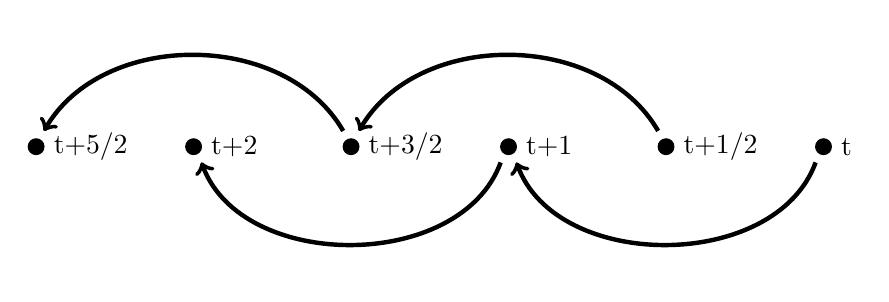
\begin{tikzpicture}[]
		\draw[<-,ultra thick] (0.1,0.2) to [out=60,in=120] (3.9,0.2);
		\draw[<-,ultra thick] (2.1,-0.2) to [out=-70,in=-110] (5.9,-0.2);
		\draw[<-,ultra thick] (4.1,0.2) to [out=60,in=120] (7.9,0.2);
		\draw[<-,ultra thick] (6.1,-0.2) to [out=-70,in=-110] (9.9,-0.2);
		\draw[fill] (0, 0) circle [radius=0.1];
		\draw[fill] (2, 0) circle [radius=0.1];
		\draw[fill] (4, 0) circle [radius=0.1];
		\draw[fill] (6, 0) circle [radius=0.1];
		\draw[fill] (8, 0) circle [radius=0.1];
		\draw[fill] (10, 0) circle [radius=0.1];
		\node [right] at (0.1,0) {t+5/2};
		\node [right] at (2.1,0) {t+2};
		\node [right] at (4.1,0) {t+3/2};
		\node [right] at (6.1,0) {t+1};
		\node [right] at (8.1,0) {t+1/2};
		\node [right] at (10.1,0) {t};	
		\end{tikzpicture}
	}
	\captionof{figure}{}
	\label{fig:time_grid}
	\end{minipage}
	And writing (\ref{eq:time_shift}) in the form
	\begin{align}
		\mathbf{r}^{t+1}_{n,m}=&\mathbf{T}(\mathbf{r}^t_{n,m};A^{t+1/2}_{n,m},B^{t+1/2}_{n,m}) \label{eq:leap_frog_shift_1} \\
		\mathbf{r}^{t+3/2}_{n,m}=&\mathbf{T}(\mathbf{r}^{t+1/2}_{n,m};A^{t+1}_{n,m},B^{t+1}_{n,m}) \label{eq:leap_frog_shift_2}
	\end{align}
	Use of equations (\ref{eq:leap_frog_shift_1}) and (\ref{eq:leap_frog_shift_2}) is indicated by lower and upper arrows in fig \ref{fig:time_grid}. To start this system we calculate $\mathbf{r}^{1/2}_{n,m}$ by using eq. (\ref{eq:time_shift}) and then shift to leap-frog method.
    \section{CUDA and CPU code}
    \section{Results and Discussion}
    
	\newpage
    \section{Additional figures}
	\pagenumbering{gobble}
	\begin{figure}[H]
	  \centering
	  \normalsize
	  % GNUPLOT: LaTeX picture with Postscript
\begingroup
  \makeatletter
  \providecommand\color[2][]{%
    \GenericError{(gnuplot) \space\space\space\@spaces}{%
      Package color not loaded in conjunction with
      terminal option `colourtext'%
    }{See the gnuplot documentation for explanation.%
    }{Either use 'blacktext' in gnuplot or load the package
      color.sty in LaTeX.}%
    \renewcommand\color[2][]{}%
  }%
  \providecommand\includegraphics[2][]{%
    \GenericError{(gnuplot) \space\space\space\@spaces}{%
      Package graphicx or graphics not loaded%
    }{See the gnuplot documentation for explanation.%
    }{The gnuplot epslatex terminal needs graphicx.sty or graphics.sty.}%
    \renewcommand\includegraphics[2][]{}%
  }%
  \providecommand\rotatebox[2]{#2}%
  \@ifundefined{ifGPcolor}{%
    \newif\ifGPcolor
    \GPcolortrue
  }{}%
  \@ifundefined{ifGPblacktext}{%
    \newif\ifGPblacktext
    \GPblacktextfalse
  }{}%
  % define a \g@addto@macro without @ in the name:
  \let\gplgaddtomacro\g@addto@macro
  % define empty templates for all commands taking text:
  \gdef\gplbacktext{}%
  \gdef\gplfronttext{}%
  \makeatother
  \ifGPblacktext
    % no textcolor at all
    \def\colorrgb#1{}%
    \def\colorgray#1{}%
  \else
    % gray or color?
    \ifGPcolor
      \def\colorrgb#1{\color[rgb]{#1}}%
      \def\colorgray#1{\color[gray]{#1}}%
      \expandafter\def\csname LTw\endcsname{\color{white}}%
      \expandafter\def\csname LTb\endcsname{\color{black}}%
      \expandafter\def\csname LTa\endcsname{\color{black}}%
      \expandafter\def\csname LT0\endcsname{\color[rgb]{1,0,0}}%
      \expandafter\def\csname LT1\endcsname{\color[rgb]{0,1,0}}%
      \expandafter\def\csname LT2\endcsname{\color[rgb]{0,0,1}}%
      \expandafter\def\csname LT3\endcsname{\color[rgb]{1,0,1}}%
      \expandafter\def\csname LT4\endcsname{\color[rgb]{0,1,1}}%
      \expandafter\def\csname LT5\endcsname{\color[rgb]{1,1,0}}%
      \expandafter\def\csname LT6\endcsname{\color[rgb]{0,0,0}}%
      \expandafter\def\csname LT7\endcsname{\color[rgb]{1,0.3,0}}%
      \expandafter\def\csname LT8\endcsname{\color[rgb]{0.5,0.5,0.5}}%
    \else
      % gray
      \def\colorrgb#1{\color{black}}%
      \def\colorgray#1{\color[gray]{#1}}%
      \expandafter\def\csname LTw\endcsname{\color{white}}%
      \expandafter\def\csname LTb\endcsname{\color{black}}%
      \expandafter\def\csname LTa\endcsname{\color{black}}%
      \expandafter\def\csname LT0\endcsname{\color{black}}%
      \expandafter\def\csname LT1\endcsname{\color{black}}%
      \expandafter\def\csname LT2\endcsname{\color{black}}%
      \expandafter\def\csname LT3\endcsname{\color{black}}%
      \expandafter\def\csname LT4\endcsname{\color{black}}%
      \expandafter\def\csname LT5\endcsname{\color{black}}%
      \expandafter\def\csname LT6\endcsname{\color{black}}%
      \expandafter\def\csname LT7\endcsname{\color{black}}%
      \expandafter\def\csname LT8\endcsname{\color{black}}%
    \fi
  \fi
  \setlength{\unitlength}{0.0500bp}%
  \begin{picture}(10080.00,6048.00)%
    \gplgaddtomacro\gplbacktext{%
      \csname LTb\endcsname%
      \put(688,512){\makebox(0,0)[r]{\strut{} 0}}%
      \csname LTb\endcsname%
      \put(688,1018){\makebox(0,0)[r]{\strut{} 0.1}}%
      \csname LTb\endcsname%
      \put(688,1523){\makebox(0,0)[r]{\strut{} 0.2}}%
      \csname LTb\endcsname%
      \put(688,2029){\makebox(0,0)[r]{\strut{} 0.3}}%
      \csname LTb\endcsname%
      \put(688,2534){\makebox(0,0)[r]{\strut{} 0.4}}%
      \csname LTb\endcsname%
      \put(688,3040){\makebox(0,0)[r]{\strut{} 0.5}}%
      \csname LTb\endcsname%
      \put(688,3545){\makebox(0,0)[r]{\strut{} 0.6}}%
      \csname LTb\endcsname%
      \put(688,4051){\makebox(0,0)[r]{\strut{} 0.7}}%
      \csname LTb\endcsname%
      \put(688,4556){\makebox(0,0)[r]{\strut{} 0.8}}%
      \csname LTb\endcsname%
      \put(688,5062){\makebox(0,0)[r]{\strut{} 0.9}}%
      \csname LTb\endcsname%
      \put(688,5567){\makebox(0,0)[r]{\strut{} 1}}%
      \csname LTb\endcsname%
      \put(784,352){\makebox(0,0){\strut{} 0}}%
      \csname LTb\endcsname%
      \put(2285,352){\makebox(0,0){\strut{} 2}}%
      \csname LTb\endcsname%
      \put(3786,352){\makebox(0,0){\strut{} 4}}%
      \csname LTb\endcsname%
      \put(5287,352){\makebox(0,0){\strut{} 6}}%
      \csname LTb\endcsname%
      \put(6788,352){\makebox(0,0){\strut{} 8}}%
      \csname LTb\endcsname%
      \put(8289,352){\makebox(0,0){\strut{} 10}}%
      \csname LTb\endcsname%
      \put(9790,352){\makebox(0,0){\strut{} 12}}%
      \put(128,3039){\rotatebox{-270}{\makebox(0,0){\strut{}$v_{dr}/v_{p}$}}}%
      \put(5287,112){\makebox(0,0){\strut{}$E_{dc}/E_{*}$}}%
      \put(5287,5807){\makebox(0,0){\strut{}$v_{dr}/v_{p}=f(E_{dc}/E_{*})$ $\mu=[1.16, 11.6, 116, 232]$ $\alpha=0.9496$ $B=4$ $E_{\omega}=0$}}%
    }%
    \gplgaddtomacro\gplfronttext{%
      \csname LTb\endcsname%
      \put(9055,5424){\makebox(0,0)[r]{\strut{}$\mu=232$}}%
      \csname LTb\endcsname%
      \put(9055,5264){\makebox(0,0)[r]{\strut{}$\mu=116$}}%
      \csname LTb\endcsname%
      \put(9055,5104){\makebox(0,0)[r]{\strut{}$\mu=11.6$}}%
      \csname LTb\endcsname%
      \put(9055,4944){\makebox(0,0)[r]{\strut{}$\mu=1.16$}}%
      \csname LTb\endcsname%
      \put(9055,4784){\makebox(0,0)[r]{\strut{}B=0 Esaki-Tsu}}%
    }%
    \gplbacktext
    \put(0,0){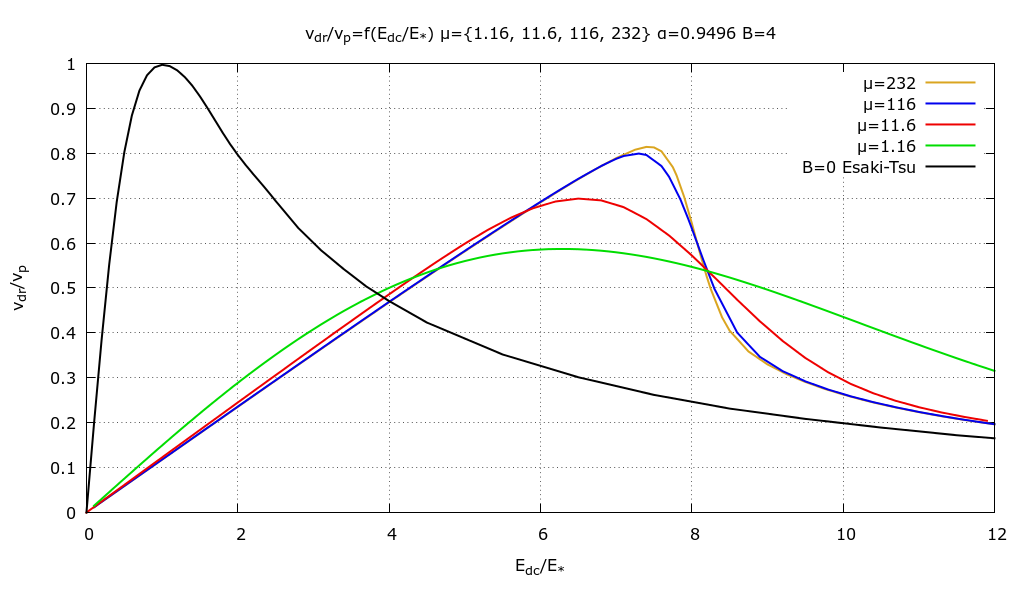
\includegraphics{v_dr_of_e_dc_B=4_mu=11_dot_6_116}}%
    \gplfronttext
  \end{picture}%
\endgroup

	  \label{fig:v_dr_of_E_dc_B=4_different_mu}
	  \caption{}
	\end{figure}
	\begin{figure}[H]
	  \centering
	  \normalsize
	  % GNUPLOT: LaTeX picture with Postscript
\begingroup
  \makeatletter
  \providecommand\color[2][]{%
    \GenericError{(gnuplot) \space\space\space\@spaces}{%
      Package color not loaded in conjunction with
      terminal option `colourtext'%
    }{See the gnuplot documentation for explanation.%
    }{Either use 'blacktext' in gnuplot or load the package
      color.sty in LaTeX.}%
    \renewcommand\color[2][]{}%
  }%
  \providecommand\includegraphics[2][]{%
    \GenericError{(gnuplot) \space\space\space\@spaces}{%
      Package graphicx or graphics not loaded%
    }{See the gnuplot documentation for explanation.%
    }{The gnuplot epslatex terminal needs graphicx.sty or graphics.sty.}%
    \renewcommand\includegraphics[2][]{}%
  }%
  \providecommand\rotatebox[2]{#2}%
  \@ifundefined{ifGPcolor}{%
    \newif\ifGPcolor
    \GPcolortrue
  }{}%
  \@ifundefined{ifGPblacktext}{%
    \newif\ifGPblacktext
    \GPblacktextfalse
  }{}%
  % define a \g@addto@macro without @ in the name:
  \let\gplgaddtomacro\g@addto@macro
  % define empty templates for all commands taking text:
  \gdef\gplbacktext{}%
  \gdef\gplfronttext{}%
  \makeatother
  \ifGPblacktext
    % no textcolor at all
    \def\colorrgb#1{}%
    \def\colorgray#1{}%
  \else
    % gray or color?
    \ifGPcolor
      \def\colorrgb#1{\color[rgb]{#1}}%
      \def\colorgray#1{\color[gray]{#1}}%
      \expandafter\def\csname LTw\endcsname{\color{white}}%
      \expandafter\def\csname LTb\endcsname{\color{black}}%
      \expandafter\def\csname LTa\endcsname{\color{black}}%
      \expandafter\def\csname LT0\endcsname{\color[rgb]{1,0,0}}%
      \expandafter\def\csname LT1\endcsname{\color[rgb]{0,1,0}}%
      \expandafter\def\csname LT2\endcsname{\color[rgb]{0,0,1}}%
      \expandafter\def\csname LT3\endcsname{\color[rgb]{1,0,1}}%
      \expandafter\def\csname LT4\endcsname{\color[rgb]{0,1,1}}%
      \expandafter\def\csname LT5\endcsname{\color[rgb]{1,1,0}}%
      \expandafter\def\csname LT6\endcsname{\color[rgb]{0,0,0}}%
      \expandafter\def\csname LT7\endcsname{\color[rgb]{1,0.3,0}}%
      \expandafter\def\csname LT8\endcsname{\color[rgb]{0.5,0.5,0.5}}%
    \else
      % gray
      \def\colorrgb#1{\color{black}}%
      \def\colorgray#1{\color[gray]{#1}}%
      \expandafter\def\csname LTw\endcsname{\color{white}}%
      \expandafter\def\csname LTb\endcsname{\color{black}}%
      \expandafter\def\csname LTa\endcsname{\color{black}}%
      \expandafter\def\csname LT0\endcsname{\color{black}}%
      \expandafter\def\csname LT1\endcsname{\color{black}}%
      \expandafter\def\csname LT2\endcsname{\color{black}}%
      \expandafter\def\csname LT3\endcsname{\color{black}}%
      \expandafter\def\csname LT4\endcsname{\color{black}}%
      \expandafter\def\csname LT5\endcsname{\color{black}}%
      \expandafter\def\csname LT6\endcsname{\color{black}}%
      \expandafter\def\csname LT7\endcsname{\color{black}}%
      \expandafter\def\csname LT8\endcsname{\color{black}}%
    \fi
  \fi
  \setlength{\unitlength}{0.0500bp}%
  \begin{picture}(10080.00,6048.00)%
    \gplgaddtomacro\gplbacktext{%
      \csname LTb\endcsname%
      \put(688,512){\makebox(0,0)[r]{\strut{}-0.4}}%
      \csname LTb\endcsname%
      \put(688,1186){\makebox(0,0)[r]{\strut{}-0.2}}%
      \csname LTb\endcsname%
      \put(688,1860){\makebox(0,0)[r]{\strut{} 0}}%
      \csname LTb\endcsname%
      \put(688,2534){\makebox(0,0)[r]{\strut{} 0.2}}%
      \csname LTb\endcsname%
      \put(688,3208){\makebox(0,0)[r]{\strut{} 0.4}}%
      \csname LTb\endcsname%
      \put(688,3882){\makebox(0,0)[r]{\strut{} 0.6}}%
      \csname LTb\endcsname%
      \put(688,4556){\makebox(0,0)[r]{\strut{} 0.8}}%
      \csname LTb\endcsname%
      \put(688,5230){\makebox(0,0)[r]{\strut{} 1}}%
      \csname LTb\endcsname%
      \put(784,352){\makebox(0,0){\strut{} 0}}%
      \csname LTb\endcsname%
      \put(2285,352){\makebox(0,0){\strut{} 2}}%
      \csname LTb\endcsname%
      \put(3786,352){\makebox(0,0){\strut{} 4}}%
      \csname LTb\endcsname%
      \put(5287,352){\makebox(0,0){\strut{} 6}}%
      \csname LTb\endcsname%
      \put(6788,352){\makebox(0,0){\strut{} 8}}%
      \csname LTb\endcsname%
      \put(8289,352){\makebox(0,0){\strut{} 10}}%
      \csname LTb\endcsname%
      \put(9790,352){\makebox(0,0){\strut{} 12}}%
      \put(128,3039){\rotatebox{-270}{\makebox(0,0){\strut{}$m/m_{x,k}$}}}%
      \put(5287,112){\makebox(0,0){\strut{}$E_{dc}/E_{*}$}}%
      \put(5287,5807){\makebox(0,0){\strut{}$m/m_{x,k}=f(E_{dc}/E_{*})$ $\mu=[1.16, 11.6, 116, 232]$ $\alpha=0.9496$ $B=4$ $E_{\omega}=0$}}%
    }%
    \gplgaddtomacro\gplfronttext{%
      \csname LTb\endcsname%
      \put(9055,5424){\makebox(0,0)[r]{\strut{}$\mu=232$}}%
      \csname LTb\endcsname%
      \put(9055,5264){\makebox(0,0)[r]{\strut{}$\mu=116$}}%
      \csname LTb\endcsname%
      \put(9055,5104){\makebox(0,0)[r]{\strut{}$\mu=11.6$}}%
      \csname LTb\endcsname%
      \put(9055,4944){\makebox(0,0)[r]{\strut{}$\mu=1.16$}}%
      \csname LTb\endcsname%
      \put(9055,4784){\makebox(0,0)[r]{\strut{}$\mu=116 B=0$}}%
    }%
    \gplbacktext
    \put(0,0){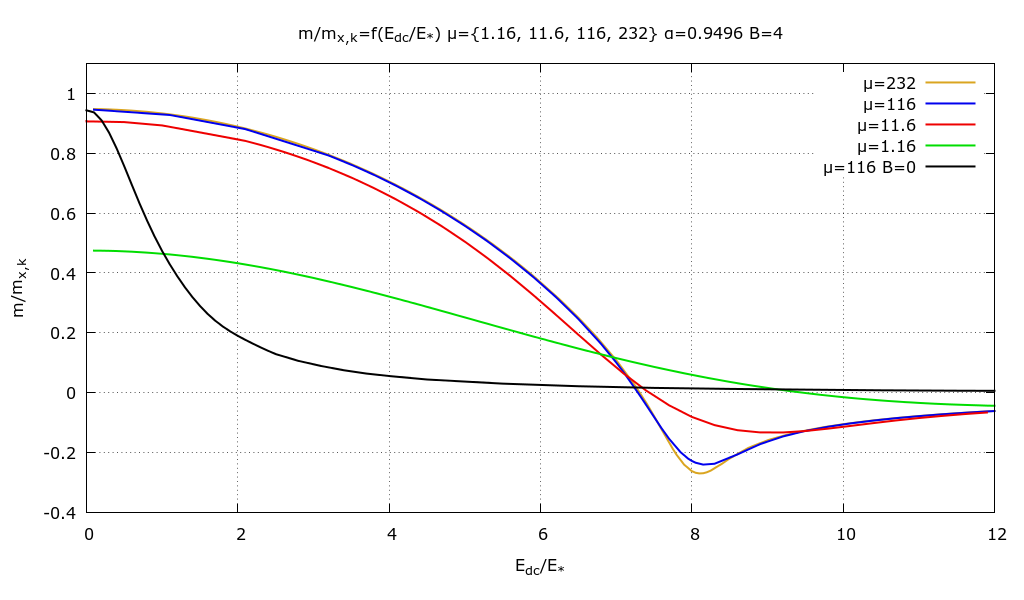
\includegraphics{m_over_m_xk_of_e_dc_B=4_mu=11_dot_6_116}}%
    \gplfronttext
  \end{picture}%
\endgroup

	  \label{fig:effect1ive_mass_of_E_dc_B=4_different_mu}
	  \caption{}
	\end{figure}
	\newpage
	\begin{figure}[t]
	  \centering
	  \normalsize % use normal font size in the figure
	  % GNUPLOT: LaTeX picture with Postscript
\begingroup
  \makeatletter
  \providecommand\color[2][]{%
    \GenericError{(gnuplot) \space\space\space\@spaces}{%
      Package color not loaded in conjunction with
      terminal option `colourtext'%
    }{See the gnuplot documentation for explanation.%
    }{Either use 'blacktext' in gnuplot or load the package
      color.sty in LaTeX.}%
    \renewcommand\color[2][]{}%
  }%
  \providecommand\includegraphics[2][]{%
    \GenericError{(gnuplot) \space\space\space\@spaces}{%
      Package graphicx or graphics not loaded%
    }{See the gnuplot documentation for explanation.%
    }{The gnuplot epslatex terminal needs graphicx.sty or graphics.sty.}%
    \renewcommand\includegraphics[2][]{}%
  }%
  \providecommand\rotatebox[2]{#2}%
  \@ifundefined{ifGPcolor}{%
    \newif\ifGPcolor
    \GPcolortrue
  }{}%
  \@ifundefined{ifGPblacktext}{%
    \newif\ifGPblacktext
    \GPblacktextfalse
  }{}%
  % define a \g@addto@macro without @ in the name:
  \let\gplgaddtomacro\g@addto@macro
  % define empty templates for all commands taking text:
  \gdef\gplbacktext{}%
  \gdef\gplfronttext{}%
  \makeatother
  \ifGPblacktext
    % no textcolor at all
    \def\colorrgb#1{}%
    \def\colorgray#1{}%
  \else
    % gray or color?
    \ifGPcolor
      \def\colorrgb#1{\color[rgb]{#1}}%
      \def\colorgray#1{\color[gray]{#1}}%
      \expandafter\def\csname LTw\endcsname{\color{white}}%
      \expandafter\def\csname LTb\endcsname{\color{black}}%
      \expandafter\def\csname LTa\endcsname{\color{black}}%
      \expandafter\def\csname LT0\endcsname{\color[rgb]{1,0,0}}%
      \expandafter\def\csname LT1\endcsname{\color[rgb]{0,1,0}}%
      \expandafter\def\csname LT2\endcsname{\color[rgb]{0,0,1}}%
      \expandafter\def\csname LT3\endcsname{\color[rgb]{1,0,1}}%
      \expandafter\def\csname LT4\endcsname{\color[rgb]{0,1,1}}%
      \expandafter\def\csname LT5\endcsname{\color[rgb]{1,1,0}}%
      \expandafter\def\csname LT6\endcsname{\color[rgb]{0,0,0}}%
      \expandafter\def\csname LT7\endcsname{\color[rgb]{1,0.3,0}}%
      \expandafter\def\csname LT8\endcsname{\color[rgb]{0.5,0.5,0.5}}%
    \else
      % gray
      \def\colorrgb#1{\color{black}}%
      \def\colorgray#1{\color[gray]{#1}}%
      \expandafter\def\csname LTw\endcsname{\color{white}}%
      \expandafter\def\csname LTb\endcsname{\color{black}}%
      \expandafter\def\csname LTa\endcsname{\color{black}}%
      \expandafter\def\csname LT0\endcsname{\color{black}}%
      \expandafter\def\csname LT1\endcsname{\color{black}}%
      \expandafter\def\csname LT2\endcsname{\color{black}}%
      \expandafter\def\csname LT3\endcsname{\color{black}}%
      \expandafter\def\csname LT4\endcsname{\color{black}}%
      \expandafter\def\csname LT5\endcsname{\color{black}}%
      \expandafter\def\csname LT6\endcsname{\color{black}}%
      \expandafter\def\csname LT7\endcsname{\color{black}}%
      \expandafter\def\csname LT8\endcsname{\color{black}}%
    \fi
  \fi
  \setlength{\unitlength}{0.0500bp}%
  \begin{picture}(10080.00,6048.00)%
    \gplgaddtomacro\gplbacktext{%
      \csname LTb\endcsname%
      \put(688,512){\makebox(0,0)[r]{\strut{} 0}}%
      \csname LTb\endcsname%
      \put(688,1018){\makebox(0,0)[r]{\strut{} 0.1}}%
      \csname LTb\endcsname%
      \put(688,1523){\makebox(0,0)[r]{\strut{} 0.2}}%
      \csname LTb\endcsname%
      \put(688,2029){\makebox(0,0)[r]{\strut{} 0.3}}%
      \csname LTb\endcsname%
      \put(688,2534){\makebox(0,0)[r]{\strut{} 0.4}}%
      \csname LTb\endcsname%
      \put(688,3040){\makebox(0,0)[r]{\strut{} 0.5}}%
      \csname LTb\endcsname%
      \put(688,3545){\makebox(0,0)[r]{\strut{} 0.6}}%
      \csname LTb\endcsname%
      \put(688,4051){\makebox(0,0)[r]{\strut{} 0.7}}%
      \csname LTb\endcsname%
      \put(688,4556){\makebox(0,0)[r]{\strut{} 0.8}}%
      \csname LTb\endcsname%
      \put(688,5062){\makebox(0,0)[r]{\strut{} 0.9}}%
      \csname LTb\endcsname%
      \put(688,5567){\makebox(0,0)[r]{\strut{} 1}}%
      \csname LTb\endcsname%
      \put(784,352){\makebox(0,0){\strut{} 0}}%
      \csname LTb\endcsname%
      \put(1763,352){\makebox(0,0){\strut{} 2}}%
      \csname LTb\endcsname%
      \put(2742,352){\makebox(0,0){\strut{} 4}}%
      \csname LTb\endcsname%
      \put(3721,352){\makebox(0,0){\strut{} 6}}%
      \csname LTb\endcsname%
      \put(4700,352){\makebox(0,0){\strut{} 8}}%
      \csname LTb\endcsname%
      \put(5679,352){\makebox(0,0){\strut{} 10}}%
      \csname LTb\endcsname%
      \put(6657,352){\makebox(0,0){\strut{} 12}}%
      \csname LTb\endcsname%
      \put(7636,352){\makebox(0,0){\strut{} 14}}%
      \csname LTb\endcsname%
      \put(8615,352){\makebox(0,0){\strut{} 16}}%
      \csname LTb\endcsname%
      \put(9594,352){\makebox(0,0){\strut{} 18}}%
      \put(128,3039){\rotatebox{-270}{\makebox(0,0){\strut{}$v_{dr}/v_{p}$}}}%
      \put(5287,112){\makebox(0,0){\strut{}$E_{dc}/E_{*}$}}%
      \put(5287,5807){\makebox(0,0){\strut{}$v_{dr}/v_{p}=f(E_{dc}/E_{*})$ $\mu=116$ $\alpha=0.9496$ $B=[0, 4, 8]$ $E_{\omega}=0$}}%
    }%
    \gplgaddtomacro\gplfronttext{%
      \csname LTb\endcsname%
      \put(9055,5424){\makebox(0,0)[r]{\strut{}B=8}}%
      \csname LTb\endcsname%
      \put(9055,5264){\makebox(0,0)[r]{\strut{}B=4}}%
      \csname LTb\endcsname%
      \put(9055,5104){\makebox(0,0)[r]{\strut{}B=0 Esaki-Tsu}}%
    }%
    \gplbacktext
    \put(0,0){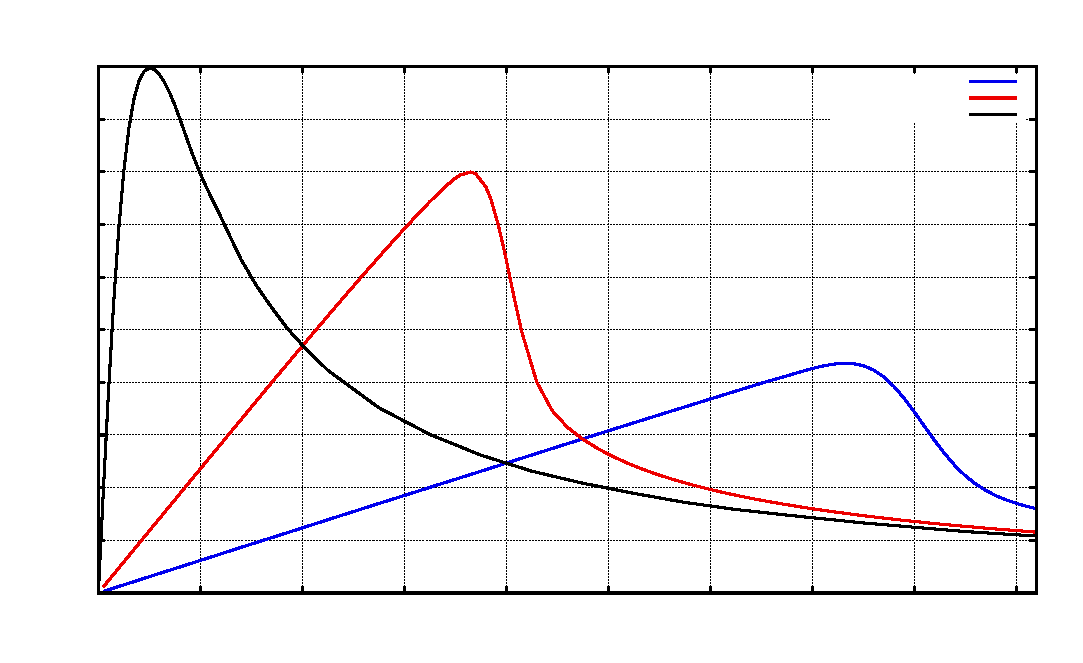
\includegraphics{v_dr_of_e_dc_B=diff}}%
    \gplfronttext
  \end{picture}%
\endgroup

	  \label{fig:v_dr_of_E_dc_different_B}
	  \caption{}
	\end{figure}
	\begin{figure}[H]
	  \centering
	  \normalsize % use normal font size in the figure
	  % GNUPLOT: LaTeX picture with Postscript
\begingroup
  \makeatletter
  \providecommand\color[2][]{%
    \GenericError{(gnuplot) \space\space\space\@spaces}{%
      Package color not loaded in conjunction with
      terminal option `colourtext'%
    }{See the gnuplot documentation for explanation.%
    }{Either use 'blacktext' in gnuplot or load the package
      color.sty in LaTeX.}%
    \renewcommand\color[2][]{}%
  }%
  \providecommand\includegraphics[2][]{%
    \GenericError{(gnuplot) \space\space\space\@spaces}{%
      Package graphicx or graphics not loaded%
    }{See the gnuplot documentation for explanation.%
    }{The gnuplot epslatex terminal needs graphicx.sty or graphics.sty.}%
    \renewcommand\includegraphics[2][]{}%
  }%
  \providecommand\rotatebox[2]{#2}%
  \@ifundefined{ifGPcolor}{%
    \newif\ifGPcolor
    \GPcolortrue
  }{}%
  \@ifundefined{ifGPblacktext}{%
    \newif\ifGPblacktext
    \GPblacktextfalse
  }{}%
  % define a \g@addto@macro without @ in the name:
  \let\gplgaddtomacro\g@addto@macro
  % define empty templates for all commands taking text:
  \gdef\gplbacktext{}%
  \gdef\gplfronttext{}%
  \makeatother
  \ifGPblacktext
    % no textcolor at all
    \def\colorrgb#1{}%
    \def\colorgray#1{}%
  \else
    % gray or color?
    \ifGPcolor
      \def\colorrgb#1{\color[rgb]{#1}}%
      \def\colorgray#1{\color[gray]{#1}}%
      \expandafter\def\csname LTw\endcsname{\color{white}}%
      \expandafter\def\csname LTb\endcsname{\color{black}}%
      \expandafter\def\csname LTa\endcsname{\color{black}}%
      \expandafter\def\csname LT0\endcsname{\color[rgb]{1,0,0}}%
      \expandafter\def\csname LT1\endcsname{\color[rgb]{0,1,0}}%
      \expandafter\def\csname LT2\endcsname{\color[rgb]{0,0,1}}%
      \expandafter\def\csname LT3\endcsname{\color[rgb]{1,0,1}}%
      \expandafter\def\csname LT4\endcsname{\color[rgb]{0,1,1}}%
      \expandafter\def\csname LT5\endcsname{\color[rgb]{1,1,0}}%
      \expandafter\def\csname LT6\endcsname{\color[rgb]{0,0,0}}%
      \expandafter\def\csname LT7\endcsname{\color[rgb]{1,0.3,0}}%
      \expandafter\def\csname LT8\endcsname{\color[rgb]{0.5,0.5,0.5}}%
    \else
      % gray
      \def\colorrgb#1{\color{black}}%
      \def\colorgray#1{\color[gray]{#1}}%
      \expandafter\def\csname LTw\endcsname{\color{white}}%
      \expandafter\def\csname LTb\endcsname{\color{black}}%
      \expandafter\def\csname LTa\endcsname{\color{black}}%
      \expandafter\def\csname LT0\endcsname{\color{black}}%
      \expandafter\def\csname LT1\endcsname{\color{black}}%
      \expandafter\def\csname LT2\endcsname{\color{black}}%
      \expandafter\def\csname LT3\endcsname{\color{black}}%
      \expandafter\def\csname LT4\endcsname{\color{black}}%
      \expandafter\def\csname LT5\endcsname{\color{black}}%
      \expandafter\def\csname LT6\endcsname{\color{black}}%
      \expandafter\def\csname LT7\endcsname{\color{black}}%
      \expandafter\def\csname LT8\endcsname{\color{black}}%
    \fi
  \fi
  \setlength{\unitlength}{0.0500bp}%
  \begin{picture}(10080.00,6048.00)%
    \gplgaddtomacro\gplbacktext{%
      \csname LTb\endcsname%
      \put(688,512){\makebox(0,0)[r]{\strut{}-0.4}}%
      \csname LTb\endcsname%
      \put(688,1186){\makebox(0,0)[r]{\strut{}-0.2}}%
      \csname LTb\endcsname%
      \put(688,1860){\makebox(0,0)[r]{\strut{} 0}}%
      \csname LTb\endcsname%
      \put(688,2534){\makebox(0,0)[r]{\strut{} 0.2}}%
      \csname LTb\endcsname%
      \put(688,3208){\makebox(0,0)[r]{\strut{} 0.4}}%
      \csname LTb\endcsname%
      \put(688,3882){\makebox(0,0)[r]{\strut{} 0.6}}%
      \csname LTb\endcsname%
      \put(688,4556){\makebox(0,0)[r]{\strut{} 0.8}}%
      \csname LTb\endcsname%
      \put(688,5230){\makebox(0,0)[r]{\strut{} 1}}%
      \csname LTb\endcsname%
      \put(784,352){\makebox(0,0){\strut{} 0}}%
      \csname LTb\endcsname%
      \put(1763,352){\makebox(0,0){\strut{} 2}}%
      \csname LTb\endcsname%
      \put(2742,352){\makebox(0,0){\strut{} 4}}%
      \csname LTb\endcsname%
      \put(3721,352){\makebox(0,0){\strut{} 6}}%
      \csname LTb\endcsname%
      \put(4700,352){\makebox(0,0){\strut{} 8}}%
      \csname LTb\endcsname%
      \put(5679,352){\makebox(0,0){\strut{} 10}}%
      \csname LTb\endcsname%
      \put(6657,352){\makebox(0,0){\strut{} 12}}%
      \csname LTb\endcsname%
      \put(7636,352){\makebox(0,0){\strut{} 14}}%
      \csname LTb\endcsname%
      \put(8615,352){\makebox(0,0){\strut{} 16}}%
      \csname LTb\endcsname%
      \put(9594,352){\makebox(0,0){\strut{} 18}}%
      \put(128,3039){\rotatebox{-270}{\makebox(0,0){\strut{}$m/m_{x,k}$}}}%
      \put(5287,112){\makebox(0,0){\strut{}$E_{dc}/E_{*}$}}%
      \put(5287,5807){\makebox(0,0){\strut{}$m/m_{x,k}=f(E_{dc}/E_{*})$ $\mu=116$ $\alpha=0.9496$ $B=[0, 4, 8]$ $E_{\omega}=0$}}%
    }%
    \gplgaddtomacro\gplfronttext{%
      \csname LTb\endcsname%
      \put(9055,5424){\makebox(0,0)[r]{\strut{}B=8}}%
      \csname LTb\endcsname%
      \put(9055,5264){\makebox(0,0)[r]{\strut{}B=4}}%
      \csname LTb\endcsname%
      \put(9055,5104){\makebox(0,0)[r]{\strut{}B=0}}%
    }%
    \gplbacktext
    \put(0,0){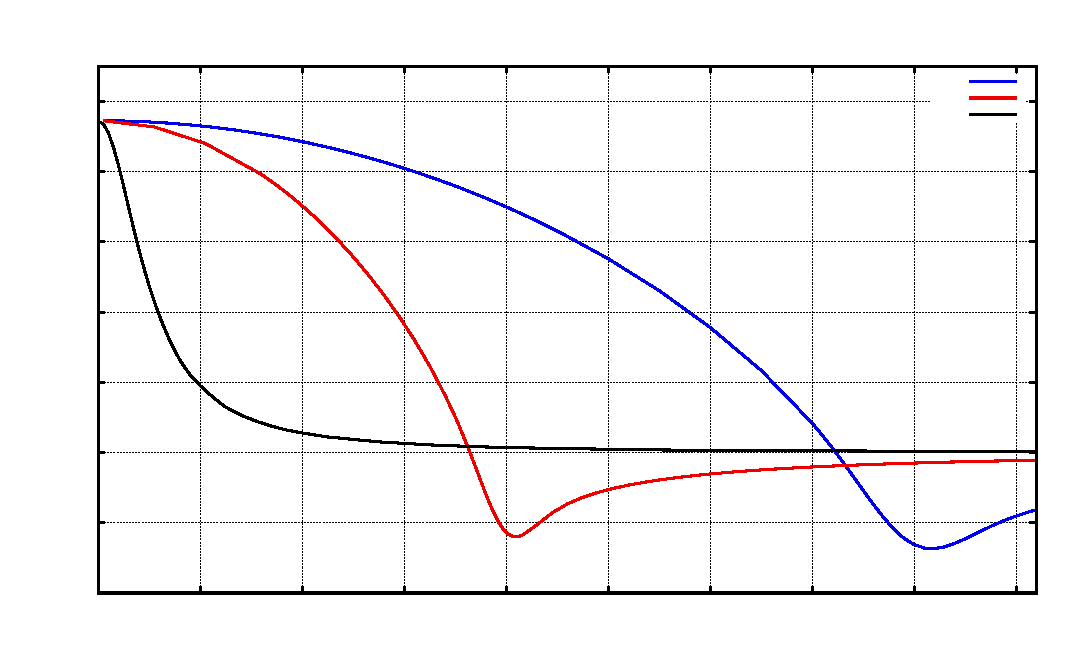
\includegraphics{m_over_m_xk_of_e_dc_B=diff}}%
    \gplfronttext
  \end{picture}%
\endgroup

	  \label{fig:effect1ive_mass_of_E_dc_different_B}
	  \caption{}
	\end{figure}
	\newpage	
%	\begin{figure}[t] %
%	  \centering
%	  \normalsize % use normal font size in the figure
%	  % GNUPLOT: LaTeX picture with Postscript
\begingroup
  \makeatletter
  \providecommand\color[2][]{%
    \GenericError{(gnuplot) \space\space\space\@spaces}{%
      Package color not loaded in conjunction with
      terminal option `colourtext'%
    }{See the gnuplot documentation for explanation.%
    }{Either use 'blacktext' in gnuplot or load the package
      color.sty in LaTeX.}%
    \renewcommand\color[2][]{}%
  }%
  \providecommand\includegraphics[2][]{%
    \GenericError{(gnuplot) \space\space\space\@spaces}{%
      Package graphicx or graphics not loaded%
    }{See the gnuplot documentation for explanation.%
    }{The gnuplot epslatex terminal needs graphicx.sty or graphics.sty.}%
    \renewcommand\includegraphics[2][]{}%
  }%
  \providecommand\rotatebox[2]{#2}%
  \@ifundefined{ifGPcolor}{%
    \newif\ifGPcolor
    \GPcolortrue
  }{}%
  \@ifundefined{ifGPblacktext}{%
    \newif\ifGPblacktext
    \GPblacktextfalse
  }{}%
  % define a \g@addto@macro without @ in the name:
  \let\gplgaddtomacro\g@addto@macro
  % define empty templates for all commands taking text:
  \gdef\gplbacktext{}%
  \gdef\gplfronttext{}%
  \makeatother
  \ifGPblacktext
    % no textcolor at all
    \def\colorrgb#1{}%
    \def\colorgray#1{}%
  \else
    % gray or color?
    \ifGPcolor
      \def\colorrgb#1{\color[rgb]{#1}}%
      \def\colorgray#1{\color[gray]{#1}}%
      \expandafter\def\csname LTw\endcsname{\color{white}}%
      \expandafter\def\csname LTb\endcsname{\color{black}}%
      \expandafter\def\csname LTa\endcsname{\color{black}}%
      \expandafter\def\csname LT0\endcsname{\color[rgb]{1,0,0}}%
      \expandafter\def\csname LT1\endcsname{\color[rgb]{0,1,0}}%
      \expandafter\def\csname LT2\endcsname{\color[rgb]{0,0,1}}%
      \expandafter\def\csname LT3\endcsname{\color[rgb]{1,0,1}}%
      \expandafter\def\csname LT4\endcsname{\color[rgb]{0,1,1}}%
      \expandafter\def\csname LT5\endcsname{\color[rgb]{1,1,0}}%
      \expandafter\def\csname LT6\endcsname{\color[rgb]{0,0,0}}%
      \expandafter\def\csname LT7\endcsname{\color[rgb]{1,0.3,0}}%
      \expandafter\def\csname LT8\endcsname{\color[rgb]{0.5,0.5,0.5}}%
    \else
      % gray
      \def\colorrgb#1{\color{black}}%
      \def\colorgray#1{\color[gray]{#1}}%
      \expandafter\def\csname LTw\endcsname{\color{white}}%
      \expandafter\def\csname LTb\endcsname{\color{black}}%
      \expandafter\def\csname LTa\endcsname{\color{black}}%
      \expandafter\def\csname LT0\endcsname{\color{black}}%
      \expandafter\def\csname LT1\endcsname{\color{black}}%
      \expandafter\def\csname LT2\endcsname{\color{black}}%
      \expandafter\def\csname LT3\endcsname{\color{black}}%
      \expandafter\def\csname LT4\endcsname{\color{black}}%
      \expandafter\def\csname LT5\endcsname{\color{black}}%
      \expandafter\def\csname LT6\endcsname{\color{black}}%
      \expandafter\def\csname LT7\endcsname{\color{black}}%
      \expandafter\def\csname LT8\endcsname{\color{black}}%
    \fi
  \fi
  \setlength{\unitlength}{0.0500bp}%
  \begin{picture}(10080.00,6048.00)%
    \gplgaddtomacro\gplbacktext{%
      \csname LTb\endcsname%
      \put(880,512){\makebox(0,0)[r]{\strut{}-0.015}}%
      \csname LTb\endcsname%
      \put(880,1152){\makebox(0,0)[r]{\strut{}-0.01}}%
      \csname LTb\endcsname%
      \put(880,1792){\makebox(0,0)[r]{\strut{}-0.005}}%
      \csname LTb\endcsname%
      \put(880,2432){\makebox(0,0)[r]{\strut{} 0}}%
      \csname LTb\endcsname%
      \put(880,3071){\makebox(0,0)[r]{\strut{} 0.005}}%
      \csname LTb\endcsname%
      \put(880,3711){\makebox(0,0)[r]{\strut{} 0.01}}%
      \csname LTb\endcsname%
      \put(880,4351){\makebox(0,0)[r]{\strut{} 0.015}}%
      \csname LTb\endcsname%
      \put(880,4991){\makebox(0,0)[r]{\strut{} 0.02}}%
      \csname LTb\endcsname%
      \put(976,352){\makebox(0,0){\strut{} 0}}%
      \csname LTb\endcsname%
      \put(2445,352){\makebox(0,0){\strut{} 2}}%
      \csname LTb\endcsname%
      \put(3914,352){\makebox(0,0){\strut{} 4}}%
      \csname LTb\endcsname%
      \put(5383,352){\makebox(0,0){\strut{} 6}}%
      \csname LTb\endcsname%
      \put(6852,352){\makebox(0,0){\strut{} 8}}%
      \csname LTb\endcsname%
      \put(8321,352){\makebox(0,0){\strut{} 10}}%
      \csname LTb\endcsname%
      \put(9790,352){\makebox(0,0){\strut{} 12}}%
      \put(128,3039){\rotatebox{-270}{\makebox(0,0){\strut{}$Absorption$}}}%
      \put(5383,112){\makebox(0,0){\strut{}$\omega$}}%
      \put(5383,5807){\makebox(0,0){\strut{}Absoprtion $A$ as a function of $\omega$. $\mu=116$ $\alpha=0.9496$ $E_{\omega}=1$ $E_{dc}=6.4$ $B=4$}}%
    }%
    \gplgaddtomacro\gplfronttext{%
      \csname LTb\endcsname%
      \put(9055,5424){\makebox(0,0)[r]{\strut{}$\mu=116$}}%
      \csname LTb\endcsname%
      \put(9055,5264){\makebox(0,0)[r]{\strut{}$\mu=1.16$}}%
    }%
    \gplbacktext
    \put(0,0){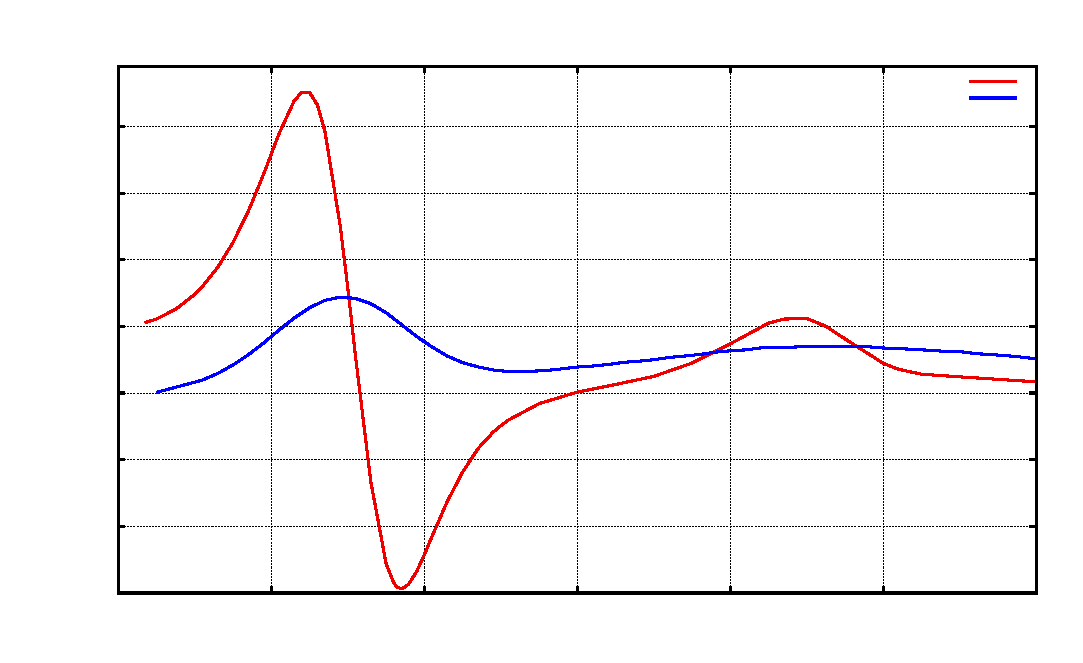
\includegraphics{combined_B=0_and_4_mu=116_and_1_16_E_omega=0_1}}%
    \gplfronttext
  \end{picture}%
\endgroup

%	  \label{fig:combined_B=0_and_4_mu=116_and_1_16_E_omega=0_1}
%	  \caption{}
%	\end{figure}		
	\begin{figure}[t]
	  \centering
	  \normalsize % use normal font size in the figure
	  % GNUPLOT: LaTeX picture with Postscript
\begingroup
  \makeatletter
  \providecommand\color[2][]{%
    \GenericError{(gnuplot) \space\space\space\@spaces}{%
      Package color not loaded in conjunction with
      terminal option `colourtext'%
    }{See the gnuplot documentation for explanation.%
    }{Either use 'blacktext' in gnuplot or load the package
      color.sty in LaTeX.}%
    \renewcommand\color[2][]{}%
  }%
  \providecommand\includegraphics[2][]{%
    \GenericError{(gnuplot) \space\space\space\@spaces}{%
      Package graphicx or graphics not loaded%
    }{See the gnuplot documentation for explanation.%
    }{The gnuplot epslatex terminal needs graphicx.sty or graphics.sty.}%
    \renewcommand\includegraphics[2][]{}%
  }%
  \providecommand\rotatebox[2]{#2}%
  \@ifundefined{ifGPcolor}{%
    \newif\ifGPcolor
    \GPcolortrue
  }{}%
  \@ifundefined{ifGPblacktext}{%
    \newif\ifGPblacktext
    \GPblacktextfalse
  }{}%
  % define a \g@addto@macro without @ in the name:
  \let\gplgaddtomacro\g@addto@macro
  % define empty templates for all commands taking text:
  \gdef\gplbacktext{}%
  \gdef\gplfronttext{}%
  \makeatother
  \ifGPblacktext
    % no textcolor at all
    \def\colorrgb#1{}%
    \def\colorgray#1{}%
  \else
    % gray or color?
    \ifGPcolor
      \def\colorrgb#1{\color[rgb]{#1}}%
      \def\colorgray#1{\color[gray]{#1}}%
      \expandafter\def\csname LTw\endcsname{\color{white}}%
      \expandafter\def\csname LTb\endcsname{\color{black}}%
      \expandafter\def\csname LTa\endcsname{\color{black}}%
      \expandafter\def\csname LT0\endcsname{\color[rgb]{1,0,0}}%
      \expandafter\def\csname LT1\endcsname{\color[rgb]{0,1,0}}%
      \expandafter\def\csname LT2\endcsname{\color[rgb]{0,0,1}}%
      \expandafter\def\csname LT3\endcsname{\color[rgb]{1,0,1}}%
      \expandafter\def\csname LT4\endcsname{\color[rgb]{0,1,1}}%
      \expandafter\def\csname LT5\endcsname{\color[rgb]{1,1,0}}%
      \expandafter\def\csname LT6\endcsname{\color[rgb]{0,0,0}}%
      \expandafter\def\csname LT7\endcsname{\color[rgb]{1,0.3,0}}%
      \expandafter\def\csname LT8\endcsname{\color[rgb]{0.5,0.5,0.5}}%
    \else
      % gray
      \def\colorrgb#1{\color{black}}%
      \def\colorgray#1{\color[gray]{#1}}%
      \expandafter\def\csname LTw\endcsname{\color{white}}%
      \expandafter\def\csname LTb\endcsname{\color{black}}%
      \expandafter\def\csname LTa\endcsname{\color{black}}%
      \expandafter\def\csname LT0\endcsname{\color{black}}%
      \expandafter\def\csname LT1\endcsname{\color{black}}%
      \expandafter\def\csname LT2\endcsname{\color{black}}%
      \expandafter\def\csname LT3\endcsname{\color{black}}%
      \expandafter\def\csname LT4\endcsname{\color{black}}%
      \expandafter\def\csname LT5\endcsname{\color{black}}%
      \expandafter\def\csname LT6\endcsname{\color{black}}%
      \expandafter\def\csname LT7\endcsname{\color{black}}%
      \expandafter\def\csname LT8\endcsname{\color{black}}%
    \fi
  \fi
  \setlength{\unitlength}{0.0500bp}%
  \begin{picture}(10080.00,6048.00)%
    \gplgaddtomacro\gplbacktext{%
      \csname LTb\endcsname%
      \put(880,512){\makebox(0,0)[r]{\strut{}-0.015}}%
      \csname LTb\endcsname%
      \put(880,1074){\makebox(0,0)[r]{\strut{}-0.01}}%
      \csname LTb\endcsname%
      \put(880,1635){\makebox(0,0)[r]{\strut{}-0.005}}%
      \csname LTb\endcsname%
      \put(880,2197){\makebox(0,0)[r]{\strut{} 0}}%
      \csname LTb\endcsname%
      \put(880,2759){\makebox(0,0)[r]{\strut{} 0.005}}%
      \csname LTb\endcsname%
      \put(880,3320){\makebox(0,0)[r]{\strut{} 0.01}}%
      \csname LTb\endcsname%
      \put(880,3882){\makebox(0,0)[r]{\strut{} 0.015}}%
      \csname LTb\endcsname%
      \put(880,4444){\makebox(0,0)[r]{\strut{} 0.02}}%
      \csname LTb\endcsname%
      \put(880,5005){\makebox(0,0)[r]{\strut{} 0.025}}%
      \csname LTb\endcsname%
      \put(880,5567){\makebox(0,0)[r]{\strut{} 0.03}}%
      \csname LTb\endcsname%
      \put(976,352){\makebox(0,0){\strut{} 0}}%
      \csname LTb\endcsname%
      \put(2445,352){\makebox(0,0){\strut{} 2}}%
      \csname LTb\endcsname%
      \put(3914,352){\makebox(0,0){\strut{} 4}}%
      \csname LTb\endcsname%
      \put(5383,352){\makebox(0,0){\strut{} 6}}%
      \csname LTb\endcsname%
      \put(6852,352){\makebox(0,0){\strut{} 8}}%
      \csname LTb\endcsname%
      \put(8321,352){\makebox(0,0){\strut{} 10}}%
      \csname LTb\endcsname%
      \put(9790,352){\makebox(0,0){\strut{} 12}}%
      \put(128,3039){\rotatebox{-270}{\makebox(0,0){\strut{}$Absorption$}}}%
      \put(5383,112){\makebox(0,0){\strut{}$\omega$}}%
      \put(5383,5807){\makebox(0,0){\strut{}Absoprtion $A$ as a function of $\omega$. $\mu=116$, $\alpha=0.9496$, $E_{\omega}=0.1$, $B=4$, $E_{dc}=[6,6.4]$}}%
    }%
    \gplgaddtomacro\gplfronttext{%
      \csname LTb\endcsname%
      \put(9055,5424){\makebox(0,0)[r]{\strut{}$E_{dc}=6.4$}}%
      \csname LTb\endcsname%
      \put(9055,5264){\makebox(0,0)[r]{\strut{}$E_{dc}=6$}}%
    }%
    \gplbacktext
    \put(0,0){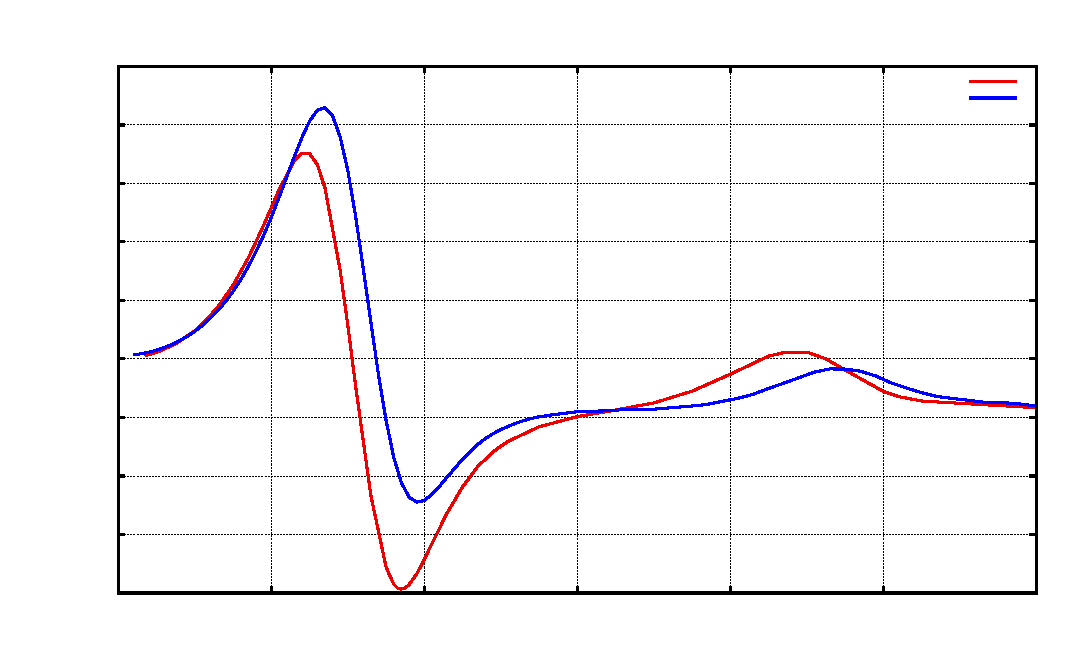
\includegraphics{combined_B=4_mu=116_E_omega=0_1_E_dc=6_vs_6_point_4}}%
    \gplfronttext
  \end{picture}%
\endgroup

	  \label{fig:combined_B=4_mu=116_E_omega=0_1_E_dc=6_vs_6_point_4}
	  \caption{}
	\end{figure}	
	\begin{figure}[H]
	  \centering
	  \normalsize % use normal font size in the figure
	  % GNUPLOT: LaTeX picture with Postscript
\begingroup
  \makeatletter
  \providecommand\color[2][]{%
    \GenericError{(gnuplot) \space\space\space\@spaces}{%
      Package color not loaded in conjunction with
      terminal option `colourtext'%
    }{See the gnuplot documentation for explanation.%
    }{Either use 'blacktext' in gnuplot or load the package
      color.sty in LaTeX.}%
    \renewcommand\color[2][]{}%
  }%
  \providecommand\includegraphics[2][]{%
    \GenericError{(gnuplot) \space\space\space\@spaces}{%
      Package graphicx or graphics not loaded%
    }{See the gnuplot documentation for explanation.%
    }{The gnuplot epslatex terminal needs graphicx.sty or graphics.sty.}%
    \renewcommand\includegraphics[2][]{}%
  }%
  \providecommand\rotatebox[2]{#2}%
  \@ifundefined{ifGPcolor}{%
    \newif\ifGPcolor
    \GPcolortrue
  }{}%
  \@ifundefined{ifGPblacktext}{%
    \newif\ifGPblacktext
    \GPblacktextfalse
  }{}%
  % define a \g@addto@macro without @ in the name:
  \let\gplgaddtomacro\g@addto@macro
  % define empty templates for all commands taking text:
  \gdef\gplbacktext{}%
  \gdef\gplfronttext{}%
  \makeatother
  \ifGPblacktext
    % no textcolor at all
    \def\colorrgb#1{}%
    \def\colorgray#1{}%
  \else
    % gray or color?
    \ifGPcolor
      \def\colorrgb#1{\color[rgb]{#1}}%
      \def\colorgray#1{\color[gray]{#1}}%
      \expandafter\def\csname LTw\endcsname{\color{white}}%
      \expandafter\def\csname LTb\endcsname{\color{black}}%
      \expandafter\def\csname LTa\endcsname{\color{black}}%
      \expandafter\def\csname LT0\endcsname{\color[rgb]{1,0,0}}%
      \expandafter\def\csname LT1\endcsname{\color[rgb]{0,1,0}}%
      \expandafter\def\csname LT2\endcsname{\color[rgb]{0,0,1}}%
      \expandafter\def\csname LT3\endcsname{\color[rgb]{1,0,1}}%
      \expandafter\def\csname LT4\endcsname{\color[rgb]{0,1,1}}%
      \expandafter\def\csname LT5\endcsname{\color[rgb]{1,1,0}}%
      \expandafter\def\csname LT6\endcsname{\color[rgb]{0,0,0}}%
      \expandafter\def\csname LT7\endcsname{\color[rgb]{1,0.3,0}}%
      \expandafter\def\csname LT8\endcsname{\color[rgb]{0.5,0.5,0.5}}%
    \else
      % gray
      \def\colorrgb#1{\color{black}}%
      \def\colorgray#1{\color[gray]{#1}}%
      \expandafter\def\csname LTw\endcsname{\color{white}}%
      \expandafter\def\csname LTb\endcsname{\color{black}}%
      \expandafter\def\csname LTa\endcsname{\color{black}}%
      \expandafter\def\csname LT0\endcsname{\color{black}}%
      \expandafter\def\csname LT1\endcsname{\color{black}}%
      \expandafter\def\csname LT2\endcsname{\color{black}}%
      \expandafter\def\csname LT3\endcsname{\color{black}}%
      \expandafter\def\csname LT4\endcsname{\color{black}}%
      \expandafter\def\csname LT5\endcsname{\color{black}}%
      \expandafter\def\csname LT6\endcsname{\color{black}}%
      \expandafter\def\csname LT7\endcsname{\color{black}}%
      \expandafter\def\csname LT8\endcsname{\color{black}}%
    \fi
  \fi
  \setlength{\unitlength}{0.0500bp}%
  \begin{picture}(10080.00,6048.00)%
    \gplgaddtomacro\gplbacktext{%
      \csname LTb\endcsname%
      \put(880,512){\makebox(0,0)[r]{\strut{}-0.015}}%
      \csname LTb\endcsname%
      \put(880,1152){\makebox(0,0)[r]{\strut{}-0.01}}%
      \csname LTb\endcsname%
      \put(880,1792){\makebox(0,0)[r]{\strut{}-0.005}}%
      \csname LTb\endcsname%
      \put(880,2432){\makebox(0,0)[r]{\strut{} 0}}%
      \csname LTb\endcsname%
      \put(880,3071){\makebox(0,0)[r]{\strut{} 0.005}}%
      \csname LTb\endcsname%
      \put(880,3711){\makebox(0,0)[r]{\strut{} 0.01}}%
      \csname LTb\endcsname%
      \put(880,4351){\makebox(0,0)[r]{\strut{} 0.015}}%
      \csname LTb\endcsname%
      \put(880,4991){\makebox(0,0)[r]{\strut{} 0.02}}%
      \csname LTb\endcsname%
      \put(976,352){\makebox(0,0){\strut{} 0}}%
      \csname LTb\endcsname%
      \put(2445,352){\makebox(0,0){\strut{} 2}}%
      \csname LTb\endcsname%
      \put(3914,352){\makebox(0,0){\strut{} 4}}%
      \csname LTb\endcsname%
      \put(5383,352){\makebox(0,0){\strut{} 6}}%
      \csname LTb\endcsname%
      \put(6852,352){\makebox(0,0){\strut{} 8}}%
      \csname LTb\endcsname%
      \put(8321,352){\makebox(0,0){\strut{} 10}}%
      \csname LTb\endcsname%
      \put(9790,352){\makebox(0,0){\strut{} 12}}%
      \put(128,3039){\rotatebox{-270}{\makebox(0,0){\strut{}$Absorption$}}}%
      \put(5383,112){\makebox(0,0){\strut{}$\omega$}}%
      \put(5383,5807){\makebox(0,0){\strut{}Absoprtion $A$ as a function of $\omega$. $\mu=116$, $\alpha=0.9496$, $E_{\omega}=0.1$, $E_{dc}=[0,6.4]$, $B=4$}}%
    }%
    \gplgaddtomacro\gplfronttext{%
      \csname LTb\endcsname%
      \put(9055,5424){\makebox(0,0)[r]{\strut{}$\mu=116, B=4$}}%
      \csname LTb\endcsname%
      \put(9055,5264){\makebox(0,0)[r]{\strut{}$\mu=116, B=0$ Bloch gain}}%
    }%
    \gplbacktext
    \put(0,0){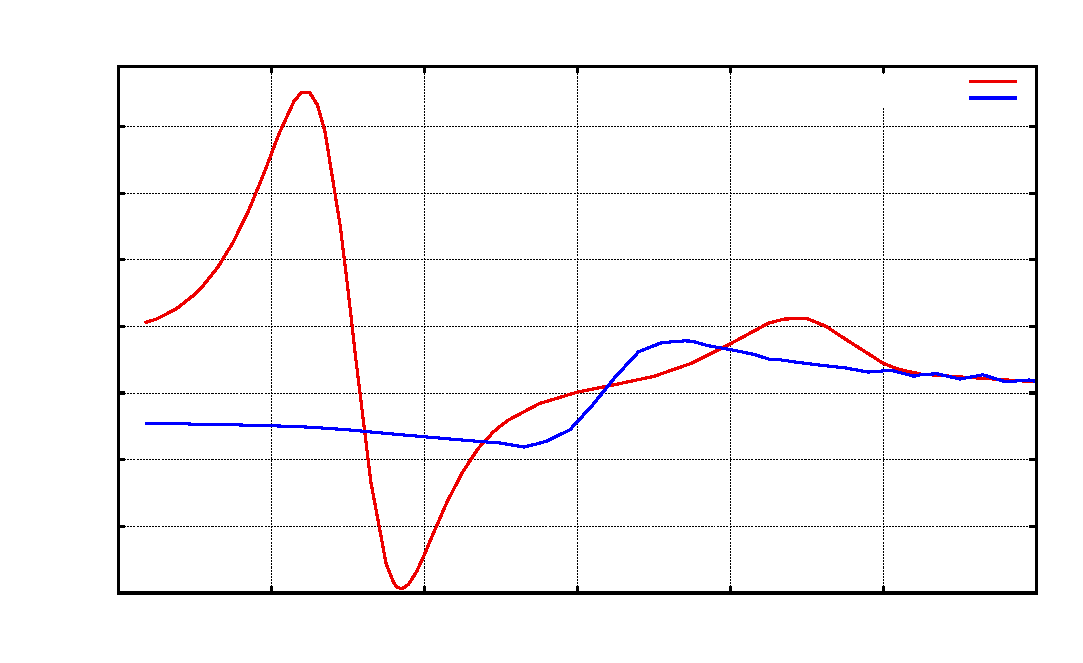
\includegraphics{cycl_vs_bloch_gain}}%
    \gplfronttext
  \end{picture}%
\endgroup

	  \label{fig:cycl_vs_bloch_gain}
	  \caption{}
	\end{figure}	
	\newpage
	\begin{figure}[t]
	  \centering
	  \normalsize % use normal font size in the figure
	  % GNUPLOT: LaTeX picture with Postscript
\begingroup
  \makeatletter
  \providecommand\color[2][]{%
    \GenericError{(gnuplot) \space\space\space\@spaces}{%
      Package color not loaded in conjunction with
      terminal option `colourtext'%
    }{See the gnuplot documentation for explanation.%
    }{Either use 'blacktext' in gnuplot or load the package
      color.sty in LaTeX.}%
    \renewcommand\color[2][]{}%
  }%
  \providecommand\includegraphics[2][]{%
    \GenericError{(gnuplot) \space\space\space\@spaces}{%
      Package graphicx or graphics not loaded%
    }{See the gnuplot documentation for explanation.%
    }{The gnuplot epslatex terminal needs graphicx.sty or graphics.sty.}%
    \renewcommand\includegraphics[2][]{}%
  }%
  \providecommand\rotatebox[2]{#2}%
  \@ifundefined{ifGPcolor}{%
    \newif\ifGPcolor
    \GPcolortrue
  }{}%
  \@ifundefined{ifGPblacktext}{%
    \newif\ifGPblacktext
    \GPblacktextfalse
  }{}%
  % define a \g@addto@macro without @ in the name:
  \let\gplgaddtomacro\g@addto@macro
  % define empty templates for all commands taking text:
  \gdef\gplbacktext{}%
  \gdef\gplfronttext{}%
  \makeatother
  \ifGPblacktext
    % no textcolor at all
    \def\colorrgb#1{}%
    \def\colorgray#1{}%
  \else
    % gray or color?
    \ifGPcolor
      \def\colorrgb#1{\color[rgb]{#1}}%
      \def\colorgray#1{\color[gray]{#1}}%
      \expandafter\def\csname LTw\endcsname{\color{white}}%
      \expandafter\def\csname LTb\endcsname{\color{black}}%
      \expandafter\def\csname LTa\endcsname{\color{black}}%
      \expandafter\def\csname LT0\endcsname{\color[rgb]{1,0,0}}%
      \expandafter\def\csname LT1\endcsname{\color[rgb]{0,1,0}}%
      \expandafter\def\csname LT2\endcsname{\color[rgb]{0,0,1}}%
      \expandafter\def\csname LT3\endcsname{\color[rgb]{1,0,1}}%
      \expandafter\def\csname LT4\endcsname{\color[rgb]{0,1,1}}%
      \expandafter\def\csname LT5\endcsname{\color[rgb]{1,1,0}}%
      \expandafter\def\csname LT6\endcsname{\color[rgb]{0,0,0}}%
      \expandafter\def\csname LT7\endcsname{\color[rgb]{1,0.3,0}}%
      \expandafter\def\csname LT8\endcsname{\color[rgb]{0.5,0.5,0.5}}%
    \else
      % gray
      \def\colorrgb#1{\color{black}}%
      \def\colorgray#1{\color[gray]{#1}}%
      \expandafter\def\csname LTw\endcsname{\color{white}}%
      \expandafter\def\csname LTb\endcsname{\color{black}}%
      \expandafter\def\csname LTa\endcsname{\color{black}}%
      \expandafter\def\csname LT0\endcsname{\color{black}}%
      \expandafter\def\csname LT1\endcsname{\color{black}}%
      \expandafter\def\csname LT2\endcsname{\color{black}}%
      \expandafter\def\csname LT3\endcsname{\color{black}}%
      \expandafter\def\csname LT4\endcsname{\color{black}}%
      \expandafter\def\csname LT5\endcsname{\color{black}}%
      \expandafter\def\csname LT6\endcsname{\color{black}}%
      \expandafter\def\csname LT7\endcsname{\color{black}}%
      \expandafter\def\csname LT8\endcsname{\color{black}}%
    \fi
  \fi
  \setlength{\unitlength}{0.0500bp}%
  \begin{picture}(10080.00,6048.00)%
    \gplgaddtomacro\gplbacktext{%
      \csname LTb\endcsname%
      \put(784,512){\makebox(0,0)[r]{\strut{} 0}}%
      \csname LTb\endcsname%
      \put(784,1466){\makebox(0,0)[r]{\strut{} 0.01}}%
      \csname LTb\endcsname%
      \put(784,2420){\makebox(0,0)[r]{\strut{} 0.02}}%
      \csname LTb\endcsname%
      \put(784,3373){\makebox(0,0)[r]{\strut{} 0.03}}%
      \csname LTb\endcsname%
      \put(784,4327){\makebox(0,0)[r]{\strut{} 0.04}}%
      \csname LTb\endcsname%
      \put(784,5281){\makebox(0,0)[r]{\strut{} 0.05}}%
      \csname LTb\endcsname%
      \put(880,352){\makebox(0,0){\strut{} 0}}%
      \csname LTb\endcsname%
      \put(2365,352){\makebox(0,0){\strut{} 2}}%
      \csname LTb\endcsname%
      \put(3850,352){\makebox(0,0){\strut{} 4}}%
      \csname LTb\endcsname%
      \put(5335,352){\makebox(0,0){\strut{} 6}}%
      \csname LTb\endcsname%
      \put(6820,352){\makebox(0,0){\strut{} 8}}%
      \csname LTb\endcsname%
      \put(8305,352){\makebox(0,0){\strut{} 10}}%
      \csname LTb\endcsname%
      \put(9790,352){\makebox(0,0){\strut{} 12}}%
      \put(128,3039){\rotatebox{-270}{\makebox(0,0){\strut{}$Absorption$}}}%
      \put(5335,112){\makebox(0,0){\strut{}$\omega$}}%
      \put(5335,5807){\makebox(0,0){\strut{}Absoprtion $A$ as a function of $\omega$. $\mu=116$, $\alpha=0.9496$, $B=4$, $E_{\omega}=0.1$, $E_{dc}=0$}}%
    }%
    \gplgaddtomacro\gplfronttext{%
      \csname LTb\endcsname%
      \put(9055,5424){\makebox(0,0)[r]{\strut{}$\mu=116$}}%
      \csname LTb\endcsname%
      \put(9055,5264){\makebox(0,0)[r]{\strut{}$\mu=\infty$}}%
    }%
    \gplbacktext
    \put(0,0){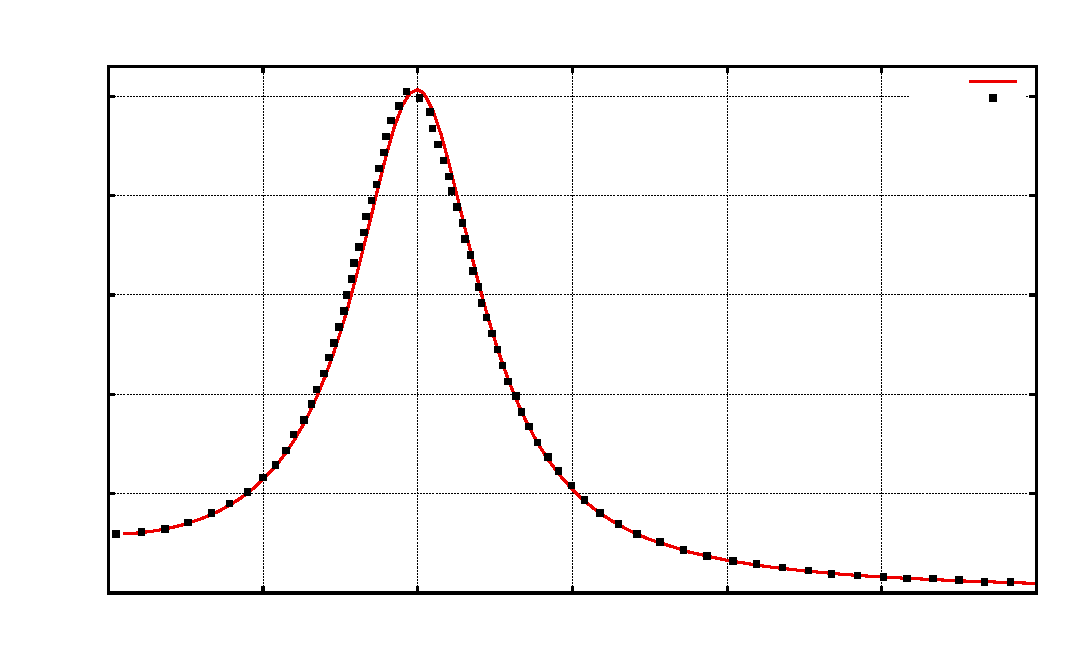
\includegraphics{lorentz_gain}}%
    \gplfronttext
  \end{picture}%
\endgroup

	  \label{fig:lorentz_gain}
	  \caption{}
	\end{figure}	
	\begin{figure}[H]
	  \centering
	  \normalsize % use normal font size in the figure
	  % GNUPLOT: LaTeX picture with Postscript
\begingroup
  \makeatletter
  \providecommand\color[2][]{%
    \GenericError{(gnuplot) \space\space\space\@spaces}{%
      Package color not loaded in conjunction with
      terminal option `colourtext'%
    }{See the gnuplot documentation for explanation.%
    }{Either use 'blacktext' in gnuplot or load the package
      color.sty in LaTeX.}%
    \renewcommand\color[2][]{}%
  }%
  \providecommand\includegraphics[2][]{%
    \GenericError{(gnuplot) \space\space\space\@spaces}{%
      Package graphicx or graphics not loaded%
    }{See the gnuplot documentation for explanation.%
    }{The gnuplot epslatex terminal needs graphicx.sty or graphics.sty.}%
    \renewcommand\includegraphics[2][]{}%
  }%
  \providecommand\rotatebox[2]{#2}%
  \@ifundefined{ifGPcolor}{%
    \newif\ifGPcolor
    \GPcolortrue
  }{}%
  \@ifundefined{ifGPblacktext}{%
    \newif\ifGPblacktext
    \GPblacktextfalse
  }{}%
  % define a \g@addto@macro without @ in the name:
  \let\gplgaddtomacro\g@addto@macro
  % define empty templates for all commands taking text:
  \gdef\gplbacktext{}%
  \gdef\gplfronttext{}%
  \makeatother
  \ifGPblacktext
    % no textcolor at all
    \def\colorrgb#1{}%
    \def\colorgray#1{}%
  \else
    % gray or color?
    \ifGPcolor
      \def\colorrgb#1{\color[rgb]{#1}}%
      \def\colorgray#1{\color[gray]{#1}}%
      \expandafter\def\csname LTw\endcsname{\color{white}}%
      \expandafter\def\csname LTb\endcsname{\color{black}}%
      \expandafter\def\csname LTa\endcsname{\color{black}}%
      \expandafter\def\csname LT0\endcsname{\color[rgb]{1,0,0}}%
      \expandafter\def\csname LT1\endcsname{\color[rgb]{0,1,0}}%
      \expandafter\def\csname LT2\endcsname{\color[rgb]{0,0,1}}%
      \expandafter\def\csname LT3\endcsname{\color[rgb]{1,0,1}}%
      \expandafter\def\csname LT4\endcsname{\color[rgb]{0,1,1}}%
      \expandafter\def\csname LT5\endcsname{\color[rgb]{1,1,0}}%
      \expandafter\def\csname LT6\endcsname{\color[rgb]{0,0,0}}%
      \expandafter\def\csname LT7\endcsname{\color[rgb]{1,0.3,0}}%
      \expandafter\def\csname LT8\endcsname{\color[rgb]{0.5,0.5,0.5}}%
    \else
      % gray
      \def\colorrgb#1{\color{black}}%
      \def\colorgray#1{\color[gray]{#1}}%
      \expandafter\def\csname LTw\endcsname{\color{white}}%
      \expandafter\def\csname LTb\endcsname{\color{black}}%
      \expandafter\def\csname LTa\endcsname{\color{black}}%
      \expandafter\def\csname LT0\endcsname{\color{black}}%
      \expandafter\def\csname LT1\endcsname{\color{black}}%
      \expandafter\def\csname LT2\endcsname{\color{black}}%
      \expandafter\def\csname LT3\endcsname{\color{black}}%
      \expandafter\def\csname LT4\endcsname{\color{black}}%
      \expandafter\def\csname LT5\endcsname{\color{black}}%
      \expandafter\def\csname LT6\endcsname{\color{black}}%
      \expandafter\def\csname LT7\endcsname{\color{black}}%
      \expandafter\def\csname LT8\endcsname{\color{black}}%
    \fi
  \fi
  \setlength{\unitlength}{0.0500bp}%
  \begin{picture}(10080.00,6048.00)%
    \gplgaddtomacro\gplbacktext{%
      \csname LTb\endcsname%
      \put(880,512){\makebox(0,0)[r]{\strut{}-0.01}}%
      \csname LTb\endcsname%
      \put(880,1144){\makebox(0,0)[r]{\strut{}-0.005}}%
      \csname LTb\endcsname%
      \put(880,1776){\makebox(0,0)[r]{\strut{} 0}}%
      \csname LTb\endcsname%
      \put(880,2408){\makebox(0,0)[r]{\strut{} 0.005}}%
      \csname LTb\endcsname%
      \put(880,3040){\makebox(0,0)[r]{\strut{} 0.01}}%
      \csname LTb\endcsname%
      \put(880,3671){\makebox(0,0)[r]{\strut{} 0.015}}%
      \csname LTb\endcsname%
      \put(880,4303){\makebox(0,0)[r]{\strut{} 0.02}}%
      \csname LTb\endcsname%
      \put(880,4935){\makebox(0,0)[r]{\strut{} 0.025}}%
      \csname LTb\endcsname%
      \put(880,5567){\makebox(0,0)[r]{\strut{} 0.03}}%
      \csname LTb\endcsname%
      \put(976,352){\makebox(0,0){\strut{} 0}}%
      \csname LTb\endcsname%
      \put(2445,352){\makebox(0,0){\strut{} 2}}%
      \csname LTb\endcsname%
      \put(3914,352){\makebox(0,0){\strut{} 4}}%
      \csname LTb\endcsname%
      \put(5383,352){\makebox(0,0){\strut{} 6}}%
      \csname LTb\endcsname%
      \put(6852,352){\makebox(0,0){\strut{} 8}}%
      \csname LTb\endcsname%
      \put(8321,352){\makebox(0,0){\strut{} 10}}%
      \csname LTb\endcsname%
      \put(9790,352){\makebox(0,0){\strut{} 12}}%
      \put(128,3039){\rotatebox{-270}{\makebox(0,0){\strut{}$Absorption$}}}%
      \put(5383,112){\makebox(0,0){\strut{}$\omega$}}%
      \put(5383,5807){\makebox(0,0){\strut{}Absoprtion $A$ as a function of $\omega$. $\mu=116$, $\alpha=0.9496$, $B=4$, $E_{\omega}=0.1$, $E_{dc}=6$}}%
    }%
    \gplgaddtomacro\gplfronttext{%
      \csname LTb\endcsname%
      \put(9055,5424){\makebox(0,0)[r]{\strut{}$\mu=116$}}%
      \csname LTb\endcsname%
      \put(9055,5264){\makebox(0,0)[r]{\strut{}$\mu=\infty$}}%
    }%
    \gplbacktext
    \put(0,0){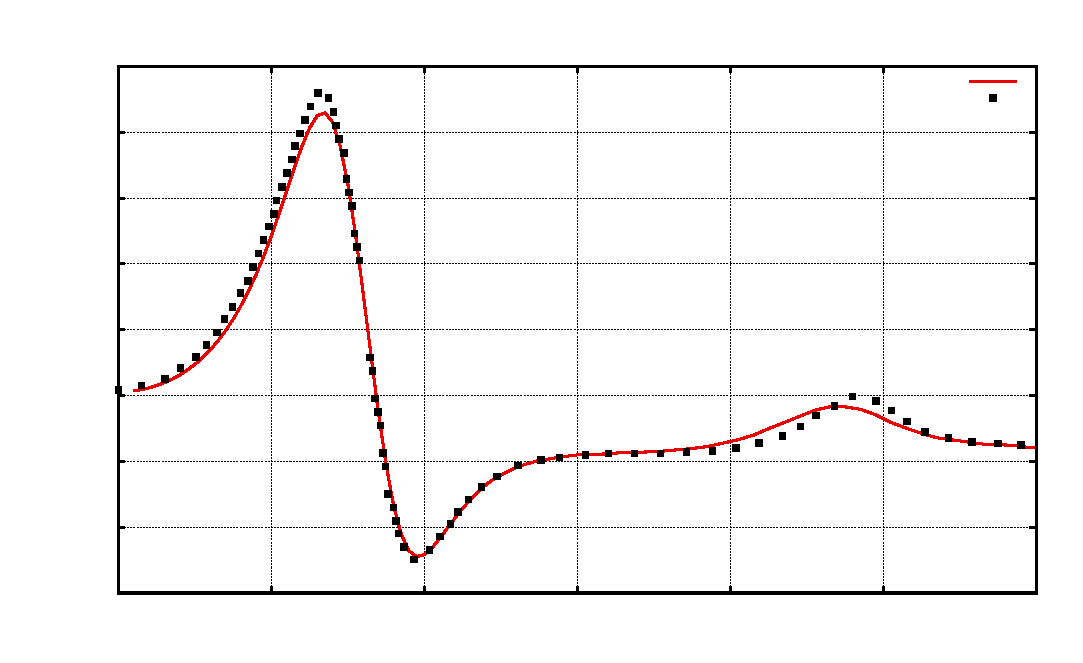
\includegraphics{gain_at_E_dc=6}}%
    \gplfronttext
  \end{picture}%
\endgroup

	  \label{fig:gain_at_E_dc=6}
	  \caption{}
	\end{figure}
	\newpage
	\begin{figure}[H]
	  \centering
	  \normalsize % use normal font size in the figure
	  \input{plots/vary_omega_B=4_mu=116_E_omega=0_1_E_dc=7_point_8}
	  \label{fig:absorption_ref_E_dc_7_point_8}
	  \caption{}
	\end{figure}	
	
	\newpage	
	\begin{figure}[t]
	  \centering
	  \normalsize % use normal font size in the figure
	  % GNUPLOT: LaTeX picture with Postscript
\begingroup
  \makeatletter
  \providecommand\color[2][]{%
    \GenericError{(gnuplot) \space\space\space\@spaces}{%
      Package color not loaded in conjunction with
      terminal option `colourtext'%
    }{See the gnuplot documentation for explanation.%
    }{Either use 'blacktext' in gnuplot or load the package
      color.sty in LaTeX.}%
    \renewcommand\color[2][]{}%
  }%
  \providecommand\includegraphics[2][]{%
    \GenericError{(gnuplot) \space\space\space\@spaces}{%
      Package graphicx or graphics not loaded%
    }{See the gnuplot documentation for explanation.%
    }{The gnuplot epslatex terminal needs graphicx.sty or graphics.sty.}%
    \renewcommand\includegraphics[2][]{}%
  }%
  \providecommand\rotatebox[2]{#2}%
  \@ifundefined{ifGPcolor}{%
    \newif\ifGPcolor
    \GPcolortrue
  }{}%
  \@ifundefined{ifGPblacktext}{%
    \newif\ifGPblacktext
    \GPblacktextfalse
  }{}%
  % define a \g@addto@macro without @ in the name:
  \let\gplgaddtomacro\g@addto@macro
  % define empty templates for all commands taking text:
  \gdef\gplbacktext{}%
  \gdef\gplfronttext{}%
  \makeatother
  \ifGPblacktext
    % no textcolor at all
    \def\colorrgb#1{}%
    \def\colorgray#1{}%
  \else
    % gray or color?
    \ifGPcolor
      \def\colorrgb#1{\color[rgb]{#1}}%
      \def\colorgray#1{\color[gray]{#1}}%
      \expandafter\def\csname LTw\endcsname{\color{white}}%
      \expandafter\def\csname LTb\endcsname{\color{black}}%
      \expandafter\def\csname LTa\endcsname{\color{black}}%
      \expandafter\def\csname LT0\endcsname{\color[rgb]{1,0,0}}%
      \expandafter\def\csname LT1\endcsname{\color[rgb]{0,1,0}}%
      \expandafter\def\csname LT2\endcsname{\color[rgb]{0,0,1}}%
      \expandafter\def\csname LT3\endcsname{\color[rgb]{1,0,1}}%
      \expandafter\def\csname LT4\endcsname{\color[rgb]{0,1,1}}%
      \expandafter\def\csname LT5\endcsname{\color[rgb]{1,1,0}}%
      \expandafter\def\csname LT6\endcsname{\color[rgb]{0,0,0}}%
      \expandafter\def\csname LT7\endcsname{\color[rgb]{1,0.3,0}}%
      \expandafter\def\csname LT8\endcsname{\color[rgb]{0.5,0.5,0.5}}%
    \else
      % gray
      \def\colorrgb#1{\color{black}}%
      \def\colorgray#1{\color[gray]{#1}}%
      \expandafter\def\csname LTw\endcsname{\color{white}}%
      \expandafter\def\csname LTb\endcsname{\color{black}}%
      \expandafter\def\csname LTa\endcsname{\color{black}}%
      \expandafter\def\csname LT0\endcsname{\color{black}}%
      \expandafter\def\csname LT1\endcsname{\color{black}}%
      \expandafter\def\csname LT2\endcsname{\color{black}}%
      \expandafter\def\csname LT3\endcsname{\color{black}}%
      \expandafter\def\csname LT4\endcsname{\color{black}}%
      \expandafter\def\csname LT5\endcsname{\color{black}}%
      \expandafter\def\csname LT6\endcsname{\color{black}}%
      \expandafter\def\csname LT7\endcsname{\color{black}}%
      \expandafter\def\csname LT8\endcsname{\color{black}}%
    \fi
  \fi
  \setlength{\unitlength}{0.0500bp}%
  \begin{picture}(14400.00,6048.00)%
    \gplgaddtomacro\gplbacktext{%
      \csname LTb\endcsname%
      \put(3960,5365){\makebox(0,0){\strut{}$E_{dc}=7.8$ $B=4$ $E_{\omega}=0.1$ $\omega=2.455$ $\mu=116$ $\alpha=0.9496$}}%
    }%
    \gplgaddtomacro\gplfronttext{%
      \csname LTb\endcsname%
      \put(721,1053){\makebox(0,0){\strut{}}}%
      \csname LTb\endcsname%
      \put(2301,1053){\makebox(0,0){\strut{}}}%
      \csname LTb\endcsname%
      \put(3881,1053){\makebox(0,0){\strut{}}}%
      \csname LTb\endcsname%
      \put(5461,1053){\makebox(0,0){\strut{}}}%
      \csname LTb\endcsname%
      \put(7041,1053){\makebox(0,0){\strut{}}}%
      \csname LTb\endcsname%
      \put(596,1334){\makebox(0,0)[r]{\strut{}-3}}%
      \csname LTb\endcsname%
      \put(596,1847){\makebox(0,0)[r]{\strut{}-2}}%
      \csname LTb\endcsname%
      \put(596,2360){\makebox(0,0)[r]{\strut{}-1}}%
      \csname LTb\endcsname%
      \put(596,2873){\makebox(0,0)[r]{\strut{} 0}}%
      \csname LTb\endcsname%
      \put(596,3386){\makebox(0,0)[r]{\strut{} 1}}%
      \csname LTb\endcsname%
      \put(596,3899){\makebox(0,0)[r]{\strut{} 2}}%
      \csname LTb\endcsname%
      \put(596,4412){\makebox(0,0)[r]{\strut{} 3}}%
      \put(356,2873){\rotatebox{-270}{\makebox(0,0){\strut{}$f(\phi_{x})$}}}%
      \put(7781,1261){\makebox(0,0)[l]{\strut{} 0}}%
      \put(7781,1583){\makebox(0,0)[l]{\strut{} 0.05}}%
      \put(7781,1905){\makebox(0,0)[l]{\strut{} 0.1}}%
      \put(7781,2228){\makebox(0,0)[l]{\strut{} 0.15}}%
      \put(7781,2550){\makebox(0,0)[l]{\strut{} 0.2}}%
      \put(7781,2873){\makebox(0,0)[l]{\strut{} 0.25}}%
      \put(7781,3195){\makebox(0,0)[l]{\strut{} 0.3}}%
      \put(7781,3517){\makebox(0,0)[l]{\strut{} 0.35}}%
      \put(7781,3840){\makebox(0,0)[l]{\strut{} 0.4}}%
      \put(7781,4162){\makebox(0,0)[l]{\strut{} 0.45}}%
      \put(7781,4485){\makebox(0,0)[l]{\strut{} 0.5}}%
    }%
    \gplgaddtomacro\gplbacktext{%
      \csname LTb\endcsname%
      \put(624,882){\makebox(0,0)[r]{\strut{} 0}}%
      \csname LTb\endcsname%
      \put(720,344){\makebox(0,0){\strut{}15}}%
      \csname LTb\endcsname%
      \put(2300,344){\makebox(0,0){\strut{}20}}%
      \csname LTb\endcsname%
      \put(3880,344){\makebox(0,0){\strut{}25}}%
      \csname LTb\endcsname%
      \put(5461,344){\makebox(0,0){\strut{}30}}%
      \csname LTb\endcsname%
      \put(7041,344){\makebox(0,0){\strut{}35}}%
      \put(416,881){\rotatebox{-270}{\makebox(0,0){\strut{}}}}%
      \put(3959,104){\makebox(0,0){\strut{}$\omega t$}}%
      \put(3959,1179){\makebox(0,0){\strut{}}}%
    }%
    \gplgaddtomacro\gplfronttext{%
    }%
    \gplbacktext
    \put(0,0){\includegraphics{plots/f_of_phi_x_and_time_A=-0_point_038_full}}%
    \gplfronttext
  \end{picture}%
\endgroup

	  \label{fig:negative_absorption_time_plot}
	  \caption{}
	\end{figure}	
	\begin{figure}[H]
	  \centering
	  \normalsize % use normal font size in the figure
	  % GNUPLOT: LaTeX picture with Postscript
\begingroup
  \makeatletter
  \providecommand\color[2][]{%
    \GenericError{(gnuplot) \space\space\space\@spaces}{%
      Package color not loaded in conjunction with
      terminal option `colourtext'%
    }{See the gnuplot documentation for explanation.%
    }{Either use 'blacktext' in gnuplot or load the package
      color.sty in LaTeX.}%
    \renewcommand\color[2][]{}%
  }%
  \providecommand\includegraphics[2][]{%
    \GenericError{(gnuplot) \space\space\space\@spaces}{%
      Package graphicx or graphics not loaded%
    }{See the gnuplot documentation for explanation.%
    }{The gnuplot epslatex terminal needs graphicx.sty or graphics.sty.}%
    \renewcommand\includegraphics[2][]{}%
  }%
  \providecommand\rotatebox[2]{#2}%
  \@ifundefined{ifGPcolor}{%
    \newif\ifGPcolor
    \GPcolortrue
  }{}%
  \@ifundefined{ifGPblacktext}{%
    \newif\ifGPblacktext
    \GPblacktextfalse
  }{}%
  % define a \g@addto@macro without @ in the name:
  \let\gplgaddtomacro\g@addto@macro
  % define empty templates for all commands taking text:
  \gdef\gplbacktext{}%
  \gdef\gplfronttext{}%
  \makeatother
  \ifGPblacktext
    % no textcolor at all
    \def\colorrgb#1{}%
    \def\colorgray#1{}%
  \else
    % gray or color?
    \ifGPcolor
      \def\colorrgb#1{\color[rgb]{#1}}%
      \def\colorgray#1{\color[gray]{#1}}%
      \expandafter\def\csname LTw\endcsname{\color{white}}%
      \expandafter\def\csname LTb\endcsname{\color{black}}%
      \expandafter\def\csname LTa\endcsname{\color{black}}%
      \expandafter\def\csname LT0\endcsname{\color[rgb]{1,0,0}}%
      \expandafter\def\csname LT1\endcsname{\color[rgb]{0,1,0}}%
      \expandafter\def\csname LT2\endcsname{\color[rgb]{0,0,1}}%
      \expandafter\def\csname LT3\endcsname{\color[rgb]{1,0,1}}%
      \expandafter\def\csname LT4\endcsname{\color[rgb]{0,1,1}}%
      \expandafter\def\csname LT5\endcsname{\color[rgb]{1,1,0}}%
      \expandafter\def\csname LT6\endcsname{\color[rgb]{0,0,0}}%
      \expandafter\def\csname LT7\endcsname{\color[rgb]{1,0.3,0}}%
      \expandafter\def\csname LT8\endcsname{\color[rgb]{0.5,0.5,0.5}}%
    \else
      % gray
      \def\colorrgb#1{\color{black}}%
      \def\colorgray#1{\color[gray]{#1}}%
      \expandafter\def\csname LTw\endcsname{\color{white}}%
      \expandafter\def\csname LTb\endcsname{\color{black}}%
      \expandafter\def\csname LTa\endcsname{\color{black}}%
      \expandafter\def\csname LT0\endcsname{\color{black}}%
      \expandafter\def\csname LT1\endcsname{\color{black}}%
      \expandafter\def\csname LT2\endcsname{\color{black}}%
      \expandafter\def\csname LT3\endcsname{\color{black}}%
      \expandafter\def\csname LT4\endcsname{\color{black}}%
      \expandafter\def\csname LT5\endcsname{\color{black}}%
      \expandafter\def\csname LT6\endcsname{\color{black}}%
      \expandafter\def\csname LT7\endcsname{\color{black}}%
      \expandafter\def\csname LT8\endcsname{\color{black}}%
    \fi
  \fi
  \setlength{\unitlength}{0.0500bp}%
  \begin{picture}(14400.00,6048.00)%
    \gplgaddtomacro\gplbacktext{%
      \csname LTb\endcsname%
      \put(3960,5365){\makebox(0,0){\strut{}$E_{dc}=7.8$ $B=4$ $E_{\omega}=0.1$ $\omega=2.455$ $\mu=116$ $\alpha=0.9496$}}%
    }%
    \gplgaddtomacro\gplfronttext{%
      \csname LTb\endcsname%
      \put(721,1053){\makebox(0,0){\strut{}}}%
      \csname LTb\endcsname%
      \put(2301,1053){\makebox(0,0){\strut{}}}%
      \csname LTb\endcsname%
      \put(3881,1053){\makebox(0,0){\strut{}}}%
      \csname LTb\endcsname%
      \put(5461,1053){\makebox(0,0){\strut{}}}%
      \csname LTb\endcsname%
      \put(7041,1053){\makebox(0,0){\strut{}}}%
      \csname LTb\endcsname%
      \put(596,1261){\makebox(0,0)[r]{\strut{} 2}}%
      \csname LTb\endcsname%
      \put(596,1826){\makebox(0,0)[r]{\strut{} 2.2}}%
      \csname LTb\endcsname%
      \put(596,2391){\makebox(0,0)[r]{\strut{} 2.4}}%
      \csname LTb\endcsname%
      \put(596,2955){\makebox(0,0)[r]{\strut{} 2.6}}%
      \csname LTb\endcsname%
      \put(596,3520){\makebox(0,0)[r]{\strut{} 2.8}}%
      \csname LTb\endcsname%
      \put(596,4085){\makebox(0,0)[r]{\strut{} 3}}%
      \put(164,2873){\rotatebox{-270}{\makebox(0,0){\strut{}$f(\phi_{x})$}}}%
      \put(7781,1261){\makebox(0,0)[l]{\strut{} 0.1}}%
      \put(7781,1664){\makebox(0,0)[l]{\strut{} 0.15}}%
      \put(7781,2067){\makebox(0,0)[l]{\strut{} 0.2}}%
      \put(7781,2470){\makebox(0,0)[l]{\strut{} 0.25}}%
      \put(7781,2873){\makebox(0,0)[l]{\strut{} 0.3}}%
      \put(7781,3275){\makebox(0,0)[l]{\strut{} 0.35}}%
      \put(7781,3678){\makebox(0,0)[l]{\strut{} 0.4}}%
      \put(7781,4081){\makebox(0,0)[l]{\strut{} 0.45}}%
      \put(7781,4484){\makebox(0,0)[l]{\strut{} 0.5}}%
    }%
    \gplgaddtomacro\gplbacktext{%
      \csname LTb\endcsname%
      \put(624,882){\makebox(0,0)[r]{\strut{} 0}}%
      \csname LTb\endcsname%
      \put(720,344){\makebox(0,0){\strut{}15}}%
      \csname LTb\endcsname%
      \put(2300,344){\makebox(0,0){\strut{}20}}%
      \csname LTb\endcsname%
      \put(3880,344){\makebox(0,0){\strut{}25}}%
      \csname LTb\endcsname%
      \put(5461,344){\makebox(0,0){\strut{}30}}%
      \csname LTb\endcsname%
      \put(7041,344){\makebox(0,0){\strut{}35}}%
      \put(416,881){\rotatebox{-270}{\makebox(0,0){\strut{}}}}%
      \put(3959,104){\makebox(0,0){\strut{}$\omega t$}}%
      \put(3959,1499){\makebox(0,0){\strut{}$E_{dc}=7.8$ $B=4$ $E_{\omega}=0.1$ $\omega=2.455$ $\mu=116$ $\alpha=0.9496$}}%
    }%
    \gplgaddtomacro\gplfronttext{%
    }%
    \gplbacktext
    \put(0,0){\includegraphics{plots/f_of_phi_x_and_time_A=-0_point_038_fragment}}%
    \gplfronttext
  \end{picture}%
\endgroup

	  \label{fig:negative_absorption_time_plot_zoom}
	  \caption{}
	\end{figure}	
	\begin{figure}[t]
	  \centering
	  \normalsize % use normal font size in the figure
	  ../../movies/vary_time/E_dc=7.8,E_omega=0.1,omega=5.1,mu=116,alpha=0.9496,B=4/plots/f_of_phi_x_and_time_A=0_point_02_full.tex
	  \label{fig:positive_absorption_time_plot}
	  \caption{}
	\end{figure}	
	\begin{figure}[H]
	  \centering
	  \normalsize % use normal font size in the figure
	  ../../movies/vary_time/E_dc=7.8,E_omega=0.1,omega=5.1,mu=116,alpha=0.9496,B=4/plots/f_of_phi_x_and_time_A=0_point_02_fragment.tex
	  \label{fig:positive_absorption_time_plot_zoom}
	  \caption{}
	\end{figure}	
	\newpage	
	\begin{figure}[t]
	  \centering
	  \normalsize % use normal font size in the figure
	  \includegraphics[scale=0.7]{plots/v_dr_and_m_vary_E_dc_and_mu.pdf}
	  \caption{$E_\omega=0.1$, $\omega=2.455$, $B=4$, $\alpha=0.9496$, $\mu=[1.16, 11.6, 116, 216]$}
	  \label{fig:effect_of_temperature_in_v_dr_vary_E_dc_omega=2.455}	  
	\end{figure}	
	\begin{figure}[H]
	  \centering
	  \normalsize % use normal font size in the figure
	  \includegraphics[scale=0.7]{plots/A_and_m_vary_E_dc_and_mu.pdf}
	  \caption{$E_\omega=0.1$, $\omega=2.455$, $B=4$, $\alpha=0.9496$, $\mu=[1.16, 11.6, 116, 216]$}
	  \label{fig:effect_of_temperature_in_A_vary_E_dc_omega=2.455}
	\end{figure}	
	\newpage	
	\begin{figure}[t]
	  \centering
	  \normalsize % use normal font size in the figure
	  \includegraphics[scale=0.7]{plots/v_dr_and_m_vary_E_dc_and_mu_omega=4.pdf}
	  \caption{$E_\omega=0.1$, $\omega=4$, $B=4$, $\alpha=0.9496$, $\mu=[1.16, 11.6, 116, 216]$}
	  \label{fig:effect_of_temperature_in_v_dr_vary_E_dc_omega=4}	  
	\end{figure}	
	\begin{figure}[H]
	  \centering
	  \normalsize % use normal font size in the figure
	  \includegraphics[scale=0.7]{plots/A_and_m_vary_E_dc_and_mu_omega=4.pdf}
	  \caption{$E_\omega=0.1$, $\omega=4$, $B=4$, $\alpha=0.9496$, $\mu=[1.16, 11.6, 116, 216]$}
	  \label{fig:effect_of_temperature_in_A_vary_E_dc_omega=4}
	\end{figure}	
	\newpage	
	\begin{figure}[t]
	  \centering
	  \normalsize % use normal font size in the figure
	  \includegraphics[scale=0.7]{plots/absorption_maps_E_omega_is_0_point_1_mu_is_116_alpha_0_point_0496.pdf}
	  \caption{Maps of absoprtion for $E_\omega=0.1$, $\alpha=0.9496$, $\mu=116$, $\tilde{B}=[1,3,4,8]$ 
	  (plots (a), (b), (c) and (d)) as a function of $\tilde{E}$ (on the x-axis) and $\omega$ (on the y-axis)}
	  \label{fig:absorption}	  
	\end{figure}	
	\begin{figure}[H]
	  \centering
	  \normalsize % use normal font size in the figure
	  \includegraphics[scale=0.7]{plots/B=4_map_and_3_A_and_Asin_plots.pdf}
	  \caption{For map of absorption (a) for $\tilde{B}=4$ we are looking at just the crossections of the
	  map showing absorption $A$ and $ASIN$ components as a functions of $\omega$ at three different values of $E_{dc}$.
	  Plot (b) corresponds to $E_{dc}=6.5$, (c) $E_{dc}=8.2$ and (d) $E_{dc}=9.5$. Line (e) corresponds to $E_{dc}=7.8$, 
	  below you will find figure \ref{fig:E_dc=7.8_B=4_different_mu} that corresponds to this line. Line (f) 
	  corresponds to $E_{dc}=7.0$, below you will find figure \ref{fig:E_dc=7.0_B=4_different_mu} that corresponds to this line.}
	  \label{fig:map_of_absorption_and_profiles_for_three_different_E_dc_B=4}
	\end{figure}	
	\newpage	
	\begin{figure}[t]
	  \centering
	  \normalsize % use normal font size in the figure
	  \includegraphics[scale=0.7]{plots/A_and_ASIN_of_omega_E_dc_is_6_point_5_vary_mu.pdf}
	  \caption{This shows effect of raising temperature on absorption and ASIN as functions of $\omega$ for parameters that 
	  correspond to Fig \ref{fig:map_of_absorption_and_profiles_for_three_different_E_dc_B=4}(b)}
	  \label{fig:E_dc=6.5_B=4_different_mu}	  
	\end{figure}
	\begin{figure}[H]
	  \centering
	  \normalsize % use normal font size in the figure
	  \includegraphics[scale=0.7]{plots/A_and_ASIN_of_omega_E_dc_is_7_point_0_vary_mu.pdf}
	  \caption{This shows effect of raising temperature on absorption and ASIN as functions of $\omega$ for parameters that 
	  correspond to Fig \ref{fig:map_of_absorption_and_profiles_for_three_different_E_dc_B=4}(f)}
	  \label{fig:E_dc=7.0_B=4_different_mu}	  
	\end{figure}
	\newpage
	\begin{figure}[t]
	  \centering
	  \normalsize % use normal font size in the figure
	  \includegraphics[scale=0.7]{plots/A_and_ASIN_of_omega_E_dc_is_7_point_8_vary_mu.pdf}
	  \caption{This shows effect of raising temperature on absorption and ASIN as functions of $\omega$ for parameters that 
	  correspond to Fig \ref{fig:map_of_absorption_and_profiles_for_three_different_E_dc_B=4}(e)}
	  \label{fig:E_dc=7.8_B=4_different_mu}	  
	\end{figure}
	\begin{figure}[H]
	  \centering
	  \normalsize % use normal font size in the figure
	  \includegraphics[scale=0.7]{plots/A_and_ASIN_of_omega_E_dc_is_8_point_2_vary_mu.pdf}
	  \caption{This shows effect of raising temperature on absorption and ASIN as functions of $\omega$ for parameters that 
	  correspond to Fig \ref{fig:map_of_absorption_and_profiles_for_three_different_E_dc_B=4}(c)}
	  \label{fig:E_dc=8.2_B=4_different_mu}	  
	\end{figure}
	\newpage
	\begin{figure}[t]
	  \centering
	  \normalsize % use normal font size in the figure
	  \includegraphics[scale=0.7]{plots/A_and_ASIN_of_omega_E_dc_is_9_point_5_vary_mu.pdf}
	  \caption{This shows effect of raising temperature on absorption and ASIN as functions of $\omega$ for parameters that 
	  correspond to Fig \ref{fig:map_of_absorption_and_profiles_for_three_different_E_dc_B=4}(d)}
	  \label{fig:E_dc=9.5_B=4_different_mu}	  
	\end{figure}
	\newpage
	\bibliography{master}
\end{document}
  
